\documentclass[a4paper,11pt]{report}
\usepackage[a4paper, total={6in, 9.5in}]{geometry}
\usepackage{cite}
\usepackage{graphicx}
\usepackage{wrapfig}
\usepackage{appendix}
\usepackage{chngcntr}
\usepackage{caption}
\usepackage{float}
\usepackage{hyperref}
\usepackage{lscape}
\usepackage{rotating}

\counterwithout{figure}{chapter}

%%%%  Add some length to the page, as margins always seem too big.  
\addtolength{\topmargin}{-.25in}

\begin{document}

%%%%  Number the initial front matter with roman numerals
\pagenumbering{roman}


%%%%  TITLE PAGE
%%  Here are the elements that make up the title page of the document.  

\thispagestyle{empty}

\title{\LARGE
ASDA Stocking Support System (Xpire)}

\author{
Luke Michael Towell
\\    \\    \\
Dissertation
\\    \\
Submitted to 
\\    \\    \\ 
The University of Liverpool
\\    \\
\\    \\
in partial fulfilment of the requirements
\\
for the degree of 
\\     \\
MASTER OF SCIENCE
\\     \\    \\    \\
}


%%  Fill in a date here if you want, or comment out the line below and
%%  the current date will be automatically inserted for you.  
\date{}


\maketitle


%%%%  ABSTRACT
\chapter*{\center Abstract}

The aim of the project is to create an application which enables ASDA colleagues to identify
and inform colleagues of which items within their fresh departments are going out of date and
need to be marked down or could potentially be provided to food shelters. The software system produced by this project will make use of mobile technology,
 backend web services and database stored procedures in order to analyse and inform colleagues which items are scheduled to go 
out of date on which date and then informs colleagues to go and reduce the products. This application
will be used throughout ASDA stores by colleagues on a daily basis and could produce a significant
cost saving and waste reduction.
\\
\\
The final products of this project will be a system of applications which will be ready for deployment
into an ASDA store in the future. The requirements and periodic demoing of the produced solution will
be provided to ASDA technology colleagues throughout the period of the project.
\\
\\
More writing about the evaluation of the project and the final outcomes. 
\newpage

\chapter*{Code Repositories}
As this project has been completed multiple code repositories have been created for each of the applications.
Each code repository contains a README.md file which provides guidance on how to run each of the applications locally on a machine. Due to the fact that all of the application have been written on a Macbook Air they have not been tested on any other Operating Systems so there may be further set up required if not running on MacOS.

\section*{Front End Applications}
\subsection*{Mobile application}
The React Native code repository - \url{https://github.com/luketowell/xpire-mobile-app}
\subsection*{Web Application}
The React code repository - \url{https://github.com/luketowell/xpire-web-application}

\section*{Back End Services}
\subsection*{Web Services}
The Java Spring-Boot repository - \url{https://github.com/luketowell/xpire-web-services}
\subsection*{Database Scripts}
All Database scripts including create and drop scripts - \url{https://github.com/luketowell/xpire_db_scripts}

\section*{Accompanying Reports}
\subsection*{Design \& Specification}
The initial report outlining the design and specification of the project. - \url{https://github.com/luketowell/COMP702-Project}
\subsection*{Final Report}
The final report which summarises project progress - \url{https://github.com/luketowell/comp702-finalReport}

%%%%  STUDENT DECLARATION ON PLAGIARISM
\chapter*{\center Student Declaration} 

I confirm that I have read and understood the University's Academic Integrity Policy.

I confirm that I have acted honestly, ethically and professionally in conduct leading
to assessment for the programme of study.  

I confirm that I have not copied material from another source nor committed plagiarism
nor fabricated data when completing the attached piece of work.  I confirm that I have 
not previously presented the work or part thereof for assessment for another University
of Liverpool module.  I confirm that I have not copied material from another source, nor
colluded with any other student in the preparation and production of this work.  

I confirm that I have not incorporated into this assignment material that has been 
submitted by me or any other person in support of a successful application for a 
degree of this or any other university or degree-awarding body.  

\vspace*{1in}

\noindent SIGNATURE \verb!______________________________________!

\noindent DATE \hspace*{.4in}  \today

\vspace*{1in}

%%  NOTE ABOUT CONFIDENTIAL MATERIAL  
%%     Students who need to keep their dissertation confidential should uncomment
%%     the following sentence on this same page.  This will preclude the dissertation 
%%     from being placed in the University Library.  Students that submit work that 
%%     isn't confidential should leave this line commented out.  

% This dissertation contains material that is confidential and/or commercially
% sensitive. It is included here on the understanding that this will not be revealed to 
% any person not involved in the assessment process.  


\newpage

%%%%  ACKNOWLEDGMENTS
%%%%    A section for Acknowledgments, should you want one.



\newpage


%%%%  TABLE OF CONTENTS  
%%%%      Usually the following command will give you the formatting you want.  

\tableofcontents


%%%%  Turn page numbering back to arabic.  This also resets the numbering
%%%%  to begin again at page 1.  

\pagenumbering{arabic}

%%%%  INTRODUCTION

\chapter{Introduction}\label{chap:intro}

\section{Summary of Project Proposal}

\subsection{Problem Statement}\label{sec:problem}
The aim of this project is to design an application and waste management system which is able
to inform store managers and store colleagues on which items of stock are going out of date or are
close to going out of date on the shop floor. This stock will then either be marked 
down on the shop floor in order to be sold on the day or will be identified as able to be donated to other charitable
causes within the local community as part of the ASDA commitment to engage and assist in the local community.
\\
\\
The key goals of the developed system are to include:
% TODO: turn into an actual list
\\
- An application which will direct colleagues to which items need to be marked down.
\\
- A reduction in store colleague hours spent in store manually marking down products.
\\
- Stock which is wasted will be reduced and identified for redistribution.
\\
\\
These goals will be assessed by peer review of colleagues in ASDA. I am also aiming to 
deploy the application in a live ASDA store with the aim of it being used in a live environment.
If I am able to deploy a POC into a live store then I will also assess the success of the 
application by comparing the product waste prior to usage in store against the wastage from 
the time that the application is used in store. 

\subsection{Project Methodology}
The methodology that I have chosen to implement for my project was a scrum agile methodology
which involved breaking the project down into smaller requirements which needed to be completed in 
iterations of development spread over the 8 weeks I developed my project in.  
\\
\\
The project included the management and development of multiple application features. Each of the features were 
detailed and documented on a Trello\cite{trello} kanban board (See Figure~\ref{fig:kanbanBoard}). 
As can be seen in Figure 1 the kanban board is broken down into "To Do", "Doing" and "Done" swim lanes.
\begin{figure}[H]
    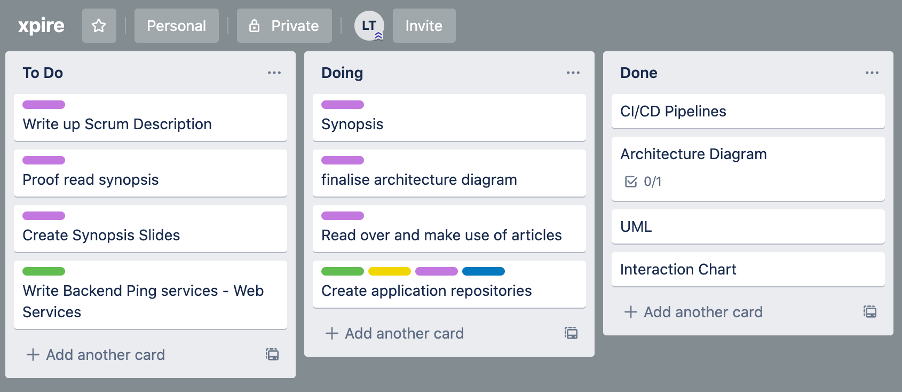
\includegraphics[width=\linewidth]{./assets/images/Kanban-board.png}
    \caption{Xpire Kanban Board}
    \label{fig:kanbanBoard}
\end{figure}

In Figure~\ref{fig:kanbanBoardFinal} you can see the updated Kanban board as I have been working on the project and moving the different requirements across the board as they have progressed.

\begin{figure}[H]
    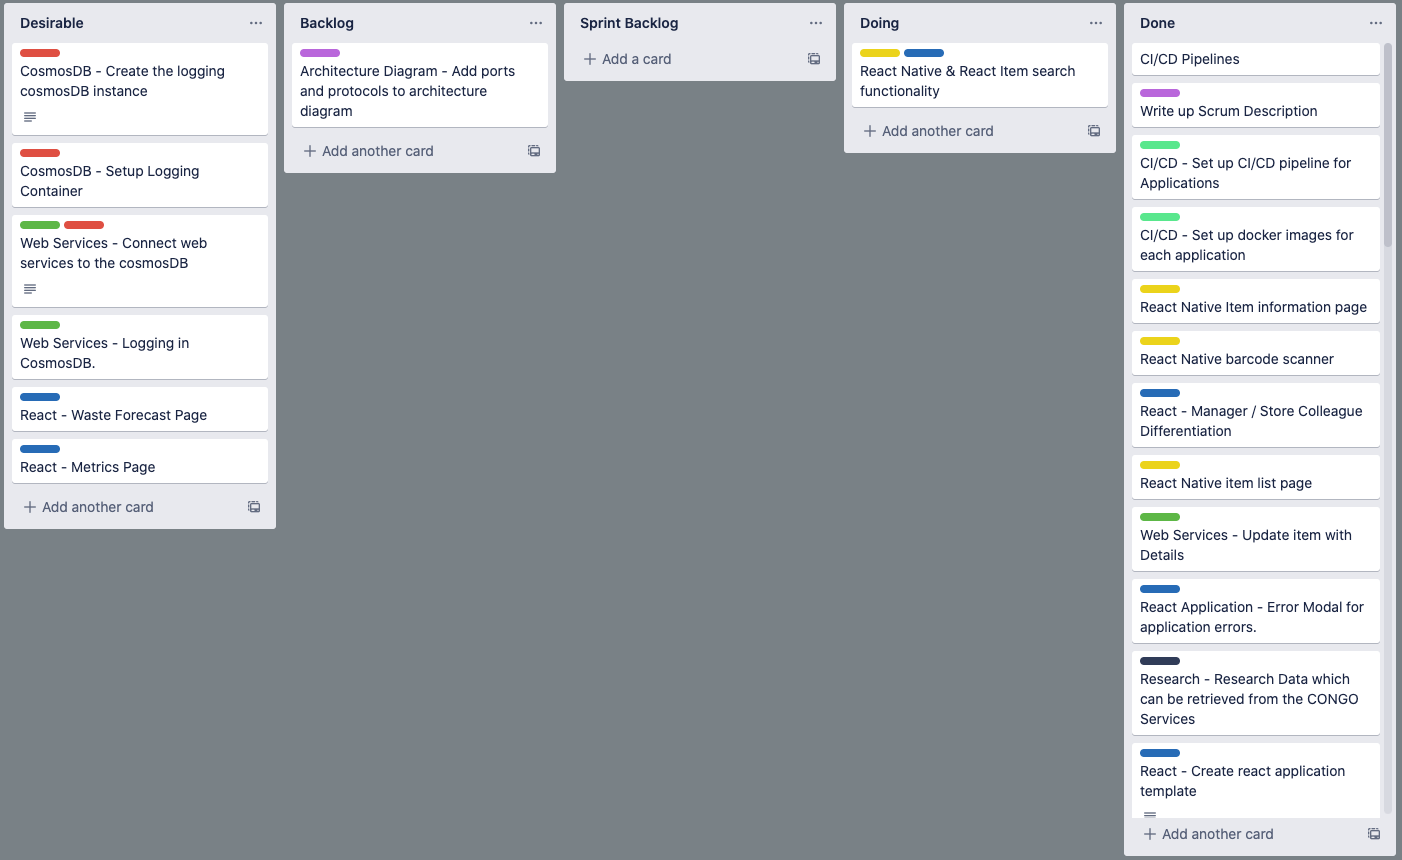
\includegraphics[width=\linewidth]{./assets/images/Kanban-2.png}
    \caption{Xpire Kanban Board - Towards completion of project.}
    \label{fig:kanbanBoardFinal}
\end{figure}

Since starting the project there have been some small changes to the way I used the Kanban board which are noticable in Figure~\ref{fig:kanbanBoardFinal}.
I have added a column to the board titled "Desirable", these are features that I have identified as being nice to have for the
project which essentially means that they are not essential to the project but could potentially add benefit if I have time to develop them.
\\
\\
I have also added labels to each of the cards so that I am easily able to identify which cards relate to each part of the application.
This has made it easier to look up which cards need working on and which features still require development. 


\chapter{Background}

At the moment sustainability and environmental responsibility are very prevelant in our day
to day lives. This ranges from the recycling which is carried out by all councils across
england to the protests and activism that takes place all across the UK by groups such 
as The Extinction Rebellion. There are regularly discussions in the media about the impact
that society and our daily habits are having on the world that we live in and what we need
to do to attempt to repair and improve our environmental impact. Wrap (Waste \& Resources Action Programme) \cite{wrapvision}
is a charity which is focused on raising public awareness of the various types of waste throughout the UK
in order to improve the use of resources in a more efficient way and to develop more sustainable products.
One of the focuses of WRAP is the food industry, WRAP highlights that approximately one third of global food
is wasted which equates to an economic loss of approximately \$984 billion globally and above £19 billion in the UK alone \cite{wrap-food-drink}.
\\
\\
It is largely accepted that we all have a part to play in assisting and improving the environment
of the planet and this is especially true for large corporations and businesses. 
\\
\\
ASDA has also focused on various schemes to be a more environmentally conscious retailer. 
These can include working with FareShare \cite{asda-food-waste} or reducing their plastics. 
\\ 
\\  
As part of the further research into the previous work others have done that is similar to my project 
I have looked for potentially similar applications which offer similar functionality to users. 
Below is an outline of the applications and a comparison against the functionality that they
offer against what my app will capable of.

\subsubsection{Too Good To Go}
Too Good To Go is an application which users are able to install on their devices.
The app displays to the user businesses which are offering their surplus food for a reduced price.
The user simply has to visit the business which is selling its reduced stock in the form of a "Magic Bag" \cite{too-good-to-go}.
\\
\\
When looking at Too Good To Go there are certainly similarities to the application that I am going to 
produce with regards to the aim of reducing waste however the main difference is that Too Good To Go 
has a focus on being the central hub for retailers to advertise their reduced produce where as the application
 I intend to produce will highlight to the user which items are going out of date. 

\subsubsection {Totalctrl}
TotalCtl is an application focused on inventory management and identifying when items are going to go out of
date which then allows the retailer, restaurant, cafe or other business to either dispose or reduce their products.
TotalCtl enables management via dashboards, graphing and alerting and is very similar application to what I am to produce\cite{totalctrl}.
\\
\\
The main difference I have identified between totalctl and my proposed solution
is that total control requires the user to upload invoices from suppliers when
items are delivered so that it can maintain its record keeping. My application 
on the other hand will make use of internal ASDA data stores, these are automatically
updated and will also enable the store to monitor stock without colleagues having to
manually enter invoices into the system.
\\
\\
Obviously the other key difference between my application and the applications discussed previously
is that my application will only deal with identifying waste that is going to go out of date within ASDA stores.
Once the stock is identified then it will be up to the colleague to decide what is done with that store following ASDA policy.
\\
\\
The main benefit of my application is that it is built bespoke for ASDA architecture and makes
use of current systems and architecture ensuring that from the beginning the application will 
work inside the ASDA ecosystem without the need for any extra development costs to make use of
a third party application. 

\section{Project requirements gathering}

As well as looking at examples of other applications which offer similar functionality to my proposed
application I also gathered requirements from ASDA employees who are familiar with the requirements 
of the project. Each of these requirements where broken down into development cards and documented on
the project Trello board. Each card contains the aim of the card, the requirement that the development
will provide and the functionality which will be available once the card has been completed. 

% TODO: insert a figure of a well documented card

% TODO: Insert notes from discussion with Philippa to document the gathering of requirements from members of the ASDA project management staff. 

% TODO: Insert potential notes from confluence. 

Through the use of the Trello board I have been able to clearly document the requirements of the applications which has allowed me to easily communicate what I am working on with the stakeholders of the system. This has assisted in meetings with ASDA colleagues when I have had to explain the development process and indicate how progress was being made.

\chapter{Ethical Use Of Data}
\section{Data used in the system}
The data used in the system will be item based information which will include a unique identifier
for an item, the expiry date / use by date of the item, the product name, the producer of the item, 
the store quantity of an item and an image of the item. 
All of this data will be available from internal ASDA databases. 
\\
\\
Other data which the application will make use of are the request details of requests 
within the system. This data is collected for the purpose of troubleshooting and monitoring
and alerting of potential issues within the application. The data will include, Request Type,
Request Content, Timestamp, Response Content, Response Information and Request Origin.
   
   
\section{Ethical Use of Data}
The data that is gathered in my application is not human related data.
The application only deals with the gathering of information on items and stores.
No user identifiable data is used therefore I have agreed with my supervisor that
there is no need to need to complete the Ethical Approval Form.
\\
\\
The only human data that will be used within this project is the feedback and opinions
of employees for ASDA which will be used in order to assess wether the goals of the 
project have been met. The consent of those whose feedback I will be using will be 
collected as and when it is required and Each individual will complete a consent form
prior to their opinions being included in the final report.


% TODO: CITE SPECIFICATION AND DESIGN DOCUMENT
\chapter{Design}
The aim of this project from the outset was to create a software system which makes use of multiple applications
 to give the in store user a clean and easy to use way of managing in-store waste. In the following chapter I 
 discuss what has been produced and what I will discuss in my dissertation.

\section{User Interface Design}

As part of the development of the system a key to ensuring the ease of use of the application was to take care and attention when
designing the user interface of the different applications. In order to do this I made use of Balsamic\cite{balsamiq} in order to design the user
interface of both the mobile and web applications. Figure~\ref{fig:UIDesignExample} shows an example of the 
interface design in Balsamiq and the final user interface that was produced. 

\subsection{Mobile Application User Interface Design}

When developing for the mobile application a key focus was the fact that I was working with a smaller screen. This meant that I needed to limit the information which is displayed on the screen whilst still providing the user with all of the information that they require. In order to do this the user flow through the application needed to be considered as well as the data which would be required by the user. ]
As you can see in Figure ~\ref{fig:UIDesignExample} the mobile application screens have been deliberately kept simple with very few options for the user to choose from. On the category screen the user is able to only view the categories that are available too them. Once the user has chosen their category then they are directed to the item list screen which filters all items which are going to expire by the category that they have chosen to ensure that the user only views the items that are applicable to their current search.

\begin{figure}[H]
    \centering
    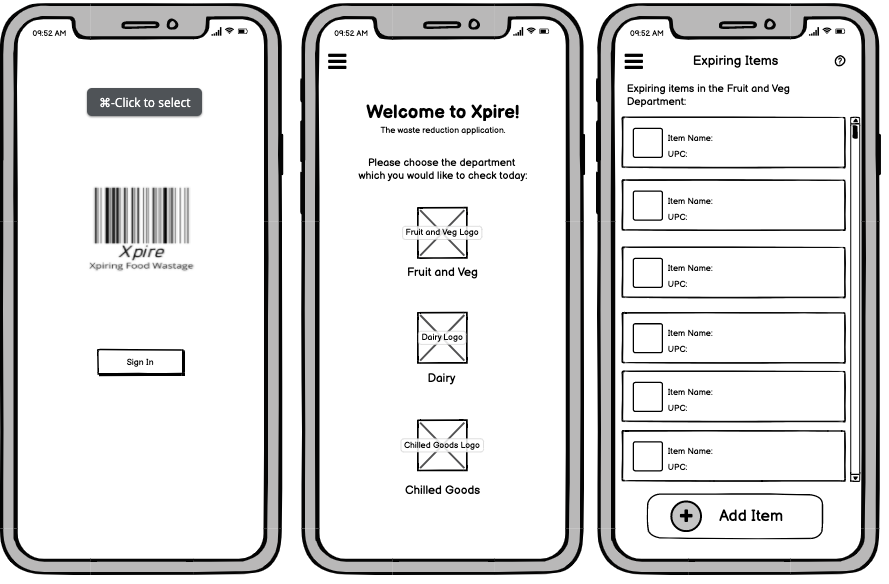
\includegraphics[width=11cm]{./assets/images/uiDesign-example.png}
    \caption{Example of the User Interface designs.}
    \label{fig:UIDesignExample}
\end{figure}

When considering the UI design of the application I wanted to also ensure that the application was visually appealing to the user and as mentioned above not overwelming. In order to achieve my aim I have had to do some research into how to design applications for mobile screens. Through my research I read various articles which stated that I should adhere to the following principles:

\begin{itemize}
    \item Navigation throughout the application should be simple.
    \item Content should be broken down into easily managable chunks of information.
    \item Input from the user should be limited to only the essential information needed from the application.
\end{itemize}

Figure ~\ref{fig:UIDesignExample} and Appendix ~\ref{appendix:mobileDesign} demonstrate that I have thought about and considered the above points when I have designed the mobile application interface. The user interface designs for the mobile application where then carried over in order to influence the design of the web application which are discussed in the following section.

\subsection{Web Application User Interface Design}

The web application is another touch point for ASDA colleagues. The main difference between the mobile application and the web application is that the web application is more likely to be used by store management and home offic staff. Due to the differing user cases there are some functionality differences between the mobile application and the web application. The main functional differences are:
\begin{itemize}
    \item User of the web application will be able to view item and expiry information for different days when using the web application.
    \item Users who are identified as management will be presented with different features which will include a metrics screen and a waste screen.
    \item Managers will also be able to change the store that they are viewing information for. 
\end{itemize}

Appendix ~\ref{appendix:webDesign} shows the designs that I created when thinking about the functionality of the application and the previous designs of the mobile application. 
It was very important that the web application has a similar design to the mobile application so that the user is able to associate each app with the other. This is in order to provide the user with a consistent experience and appearance. As can be seen with the Login, Home and Item Details screen in appendix ~\ref{appendix:webDesign} the designs and content of each of the pages are the same as those from the mobile application designs in ~\ref{appendix:mobileDesign}.

\section{Database Design}
One of the features of the system creation which took the most amount of time and research was the database.
The database schema below (See Figure ~\ref{fig:DBSchema}) shows the final design of the database including foreign key relationships, primary keys and tables.

\begin{figure}[H]
    \centering
    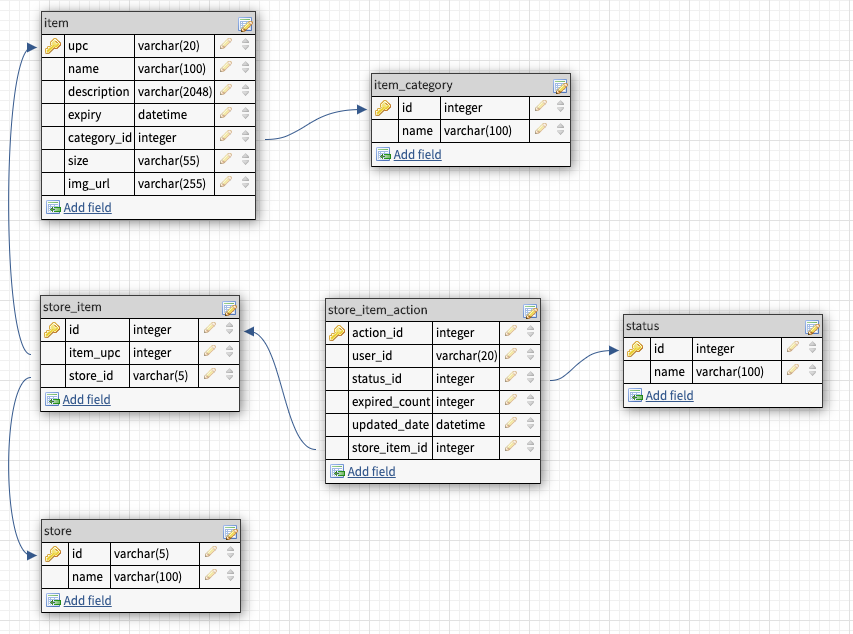
\includegraphics[width=12.5cm]{./assets/images/Database-Schema.png}
    \caption{Final database schema.}
    \label{fig:DBSchema}
\end{figure}

As you can see all of the tables are interrelated in some way with references to other tables. The main table of the database is the store{\_}item table which stores all of the relevant information needed for the store users to be able to see which items are going to expire and contains a foreign key relationship in the form of a one to one relationship with store items and item information in the item table.
\\
\\
The main actions that a user takes are then stored in the store{\_}item{\_}action table which has a many to one foreign key relationship with the store{\_}item table. this allows me to create the relationship between the store items and their relevant actions that have been recorded by users whilst also ensuring that the store items are easy to store and maintain within the DB.
\\
\\
There are three tables which have been created as they are potential options available to the user within the application. These are the item{\_}category, status and store tables which are mainly used for the creation of dropdown boxes when the user is choosing various options thoughout the application. The reason for storing the options in seperate tables within the database over hardcoding them in the application is that by abstracting the options into the database I am easily able to edit and update options without having to modify the application code which then means that I do not have to redeploy any applications or interupt any potential user flow which makes the app more user friendly for the potential users.
\\
\\
The final table is the item table. The item table contains all of the time information required for the software system. The table is populated from the large data warehouse which is used to maintain item information across the whole of the ASDA estate. Due to the security issues which I discuss in Chapter 9 I was unable to make use of tdata warehouse feed so I have had to create mock data within the item table.

\chapter{Realisation}
In the following sections I will discuss the applications which where developed as part of the Xpire system.

\section{Front End Applications}
Both of the front end applications have been written using popular javascript frameworks: React and React 
Native these are both very similar frameworks with minor differences in functionality. React is used for 
the web application which is hosted via Azure Application Hosting and can be accessed by any browser that
the user chooses. React Native has been used for the creation of the Xpire mobile application. React Native
is a framework which enables a developer to write their applications using javascript code and features of
the framework and then compile the code into Java and Swift so that the resulting IPA and APK can be ran 
on IOs or Android devices respectively.
\\
\\
I have chosen both of these frameworks for the following reasons:
\begin{itemize}
    \item The frameworks are popular javascript frameworks which I have previously used to write mobile and web applications in.
    \item Both frameworks utilise the React library meaning that the syntax of the framework is very similar. This is useful 
    when it comes to reusabilty of components and features. 
    \item Due to the popularity of each framework there are lots of additional libraries which offer additional functionality
     e.g. Barcode scanning using the device camera.
    \item There is a good wealth of documentation and support forum articles available online which enabled me to easily debug 
    and resolve any issues that I came across whilst developing the front end applications.
\end{itemize}

As well as being developed using similar frameworks both of the front end applications have been developed using similar coding standards.
 In this section I will describe what standards have been used in the front end applications and the benefits that they provide to the application code and lifecycle.

When writing both of the applications I have made use of the 12 factor app approach. The 12 factor app is a software development approach which outlines 12 practices which developers should follow in order to produce high quality applications which are easily picked up by other developers and easily expanded upon. 
Whilst developing all of my applications I have made use of environment variables in order to store application config, I have seperated the backing services into seperate web services so that they are easily manipulated without having to update the application code and I have made use of codebases which are tracked in version control in order to ensure that I am alwasy able to recall a working version of the code if I accidentally break functionality whilst developing the applications.
In the following sections I am going to go over how I have made use of the 12 factor app principles and other development principles I have made use of in order to produce high quality enterprise applications.
abstraction - use the example of the axios request
componentisation - components e.g. item card or Text component

\subsection{Mobile Application}
The mobile application of Xpire is the main part of the system which is used by the front of house store colleagues who are working on the shop floor.
The application has been written using the React-Native JavaScript framework which means that it is compatible with both android and IOs operating systems.
This means the app can be used on both in store devices as well as colleague and managers personal devices as part of the BYOD (Bring Your Own Device) scheme. 

The application is capable of communicating with the back end web services via Restful CRUD requests which ensures that all user data is as up to date as possible.
The application also includes a barcode scanner which enables users to easily scan items rather than entering relevant barcode numbers for items that they want to look up. 
\\
\\
Figure ~\ref{fig:IOSScreenshots} shows an example of the IOs version of the apps user interface. These screenshots can be directly compared against Figure ~\ref{fig:UIDesignExample}
 to show how the designs of the application have been implemented in the final versions of the application.

\begin{figure}[H]
    \centering
    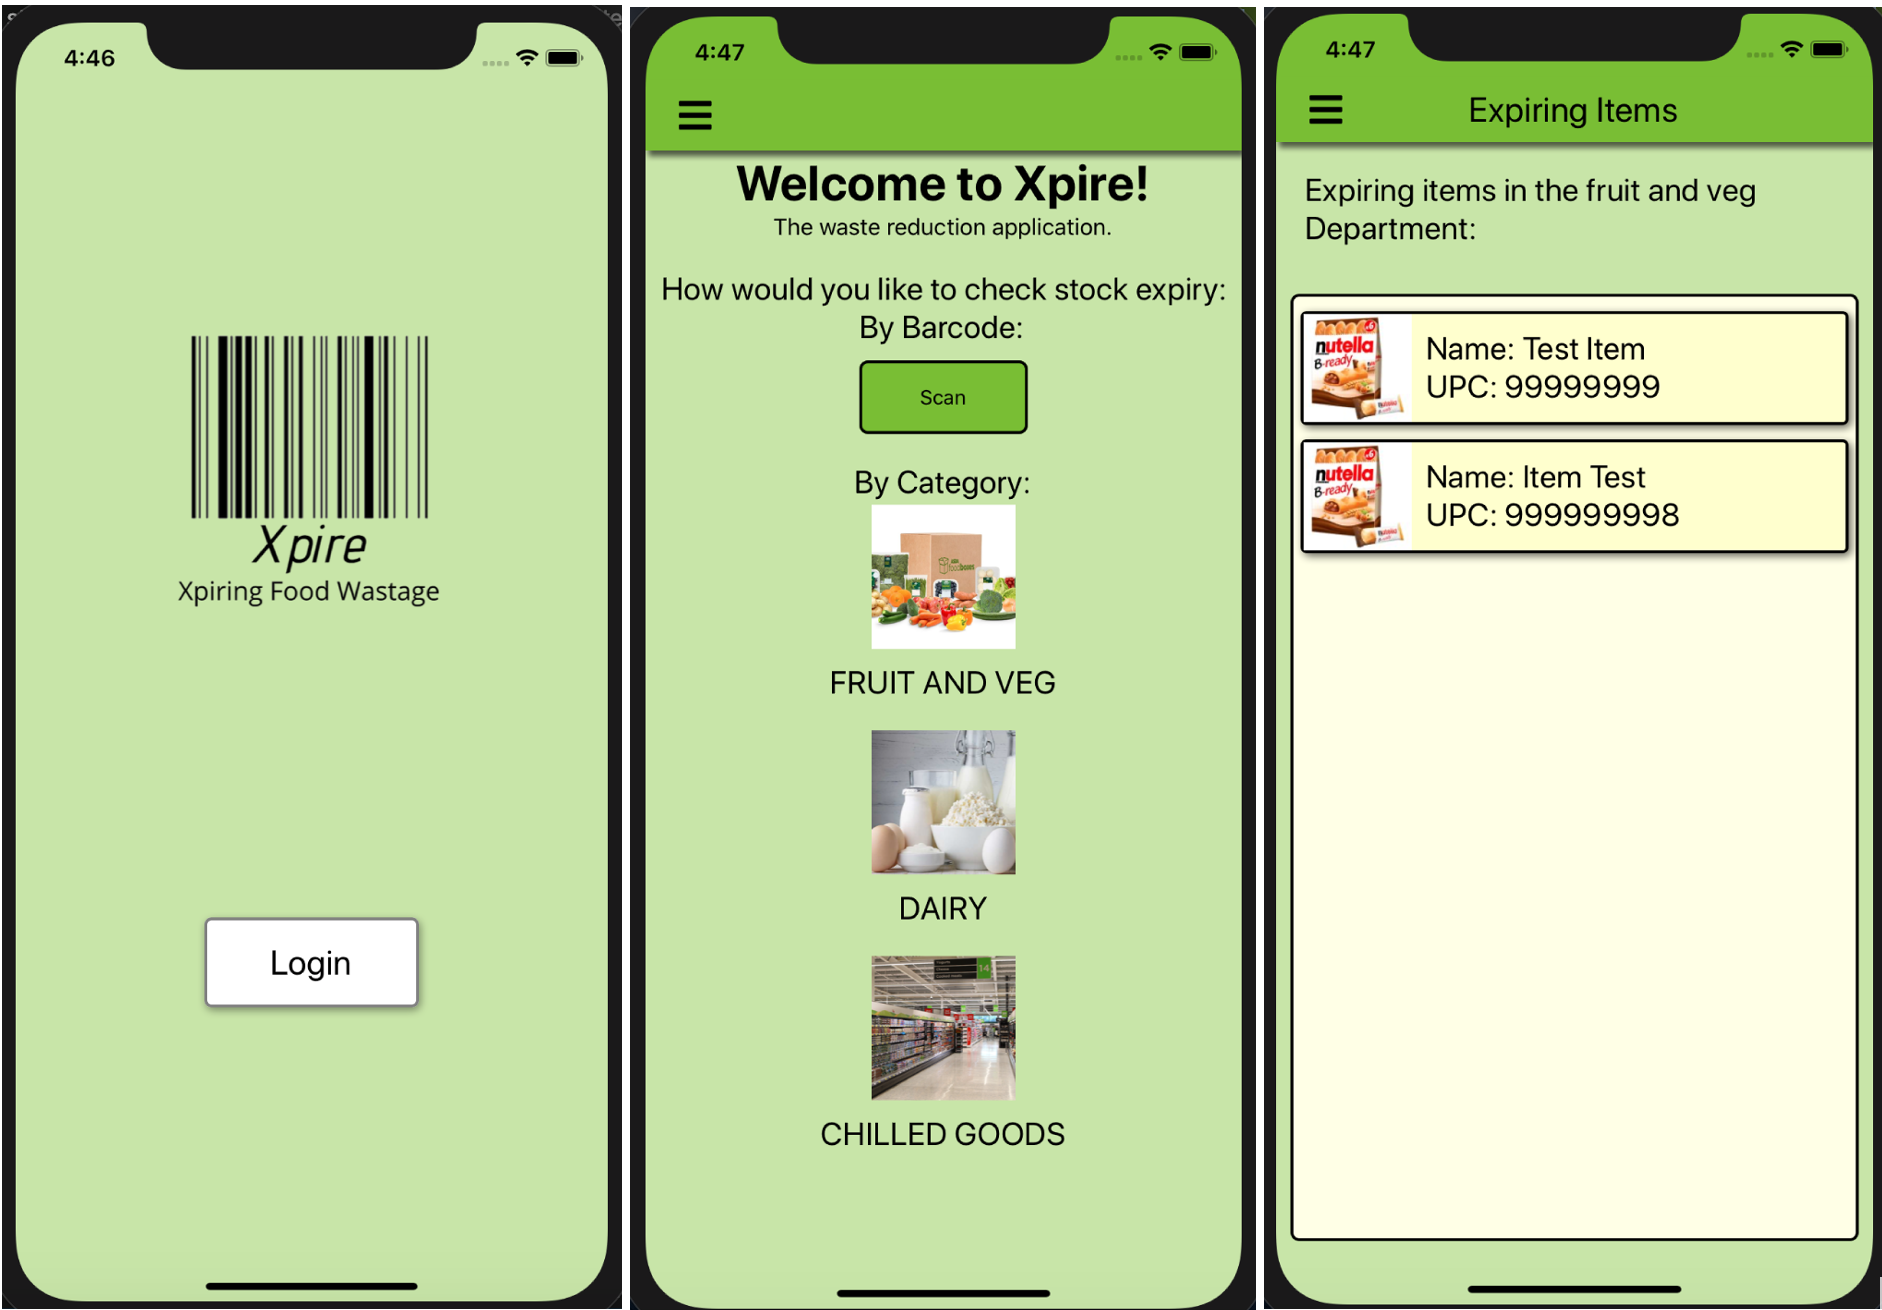
\includegraphics[width=10cm]{./assets/images/appUI.png}
    \caption{Screenshots of the IOs mobile application.}
    \label{fig:IOSScreenshots}
\end{figure}

In Appendix ~\ref{appendix:mobileUI} I have outlined three of the potential user scenarios for the application.

Here I will outline each of the user scenarios

Scenario 1


Scenario 2


Scenario 3

Development practices
As part of developing the application I have ensured that the applications are built in a way that means that the applications can be deployed within an enterprise environment. In order to do this I have made use of the 12 factor app approach which has been mentioned previously. One of the factors in the 12 factor app is the use of environmental variables in order to ensure that the applications configuration can easily be managed between different environments e.g. Dev, Stage, Production and IOs and Android. 
Figure ~\ref{fig:iosVars} shows the contents of the IOs environment variables in this file you can see the hostname of the server where the IOs application should make its requests to and the environment that the application is built for.

\begin{figure}[H]
    \centering
    \frame{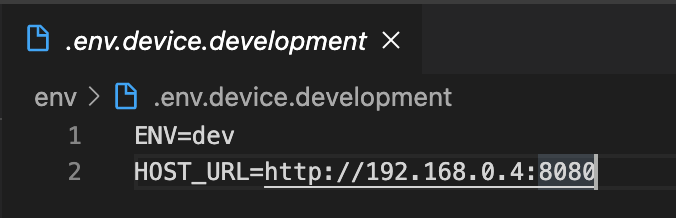
\includegraphics[width=10cm]{./assets/images/iosVars.png}}
    \caption{Content of the IOs environment variable file}
    \label{fig:iosVars}
\end{figure}

The env file is then picked up at compile time and the values are inserted into the parts of the code where the configuration is referenced. Figure ~\ref{fig:iosScript} is an example of one of the compile script which takes in the environment variable files for that particular application build.
\begin{figure}[H]
    \centering
    \frame{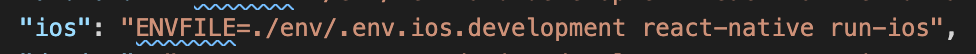
\includegraphics[width=10cm]{./assets/images/iosScript.png}}
    \caption{IOs application build file which includes the IOs environment variables.}
    \label{fig:iosScript}
\end{figure}

As well as environment variables to store configuration I have also made use of the development principle of abstraction.
Abstraction is where functionality is abstracted out from the code into a seperate module so that it can be called from
the code that requires it. Abstraction is beneficial to the code base because it means that the functionality can be reused
throughout the application without the duplication of code which would be needed if the functionality was not abstracted.
Abstraction also means that the code becomes more readable and easier to understand for other developers. 
This is because the code that the developer is reading only relates to that one function instead of potentially 
relating to multiple pieces of functionality.
\\
\\
 Figure ~\ref{fig:request} is an example of the abstraction used within both
the mobile and web applications that I have produced. I have abstracted the http request functionality into its own file 
which is then exported so that it can be imported into any other file and called from multiple locations within the application.

\begin{figure}[H]
\centering
\frame{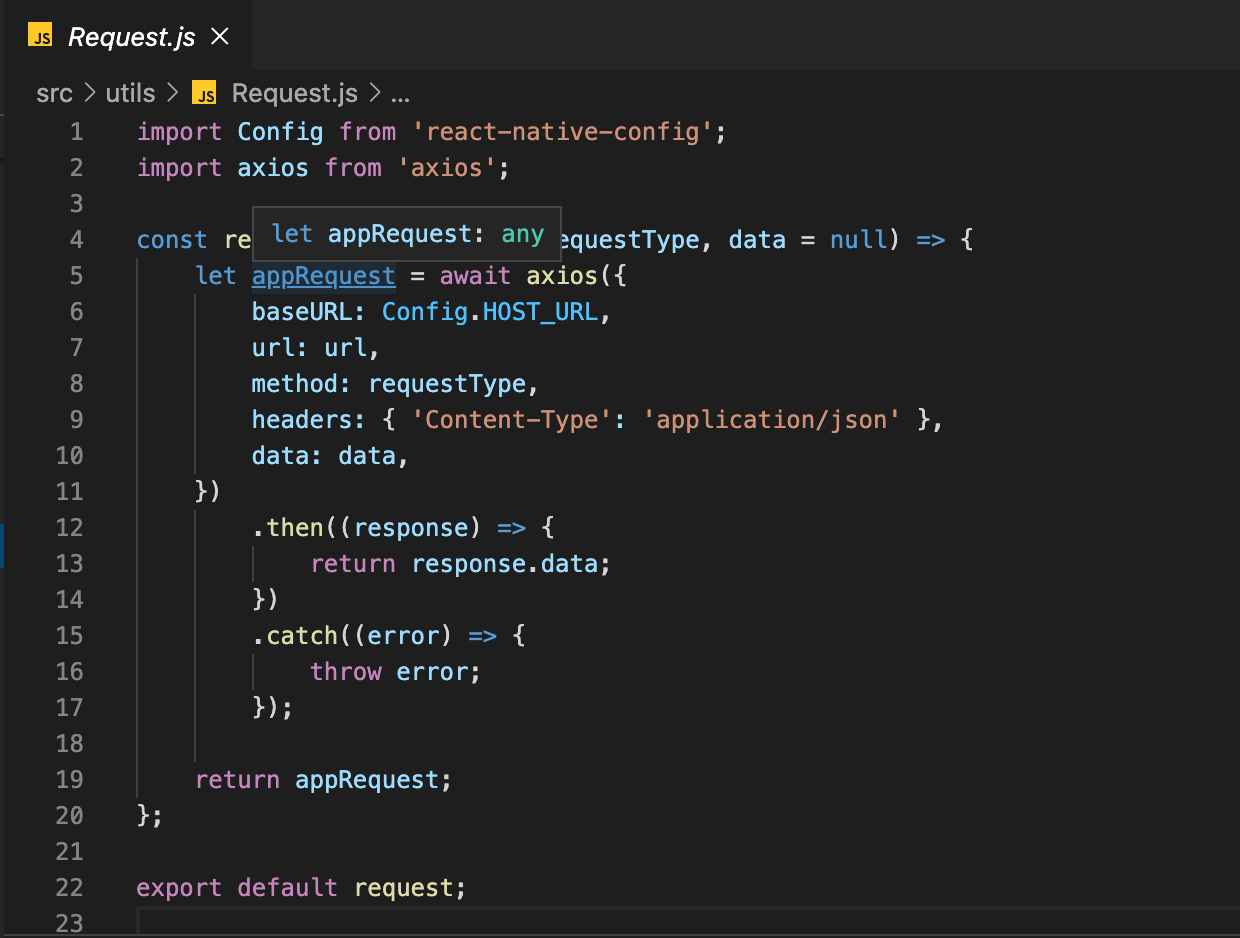
\includegraphics[width=10cm]{./assets/images/request.png}}
\caption{The http request code as an example of abstraction.}
\label{fig:request}
\end{figure}

In the request example the request function is called from any of the redux actions which want to make an http request to the
backend server. Figure  shows the action making use of the imported request functionality to make a request 
for the storeItemSummary list, this is an example of how requests to the web services are made in order to retrieve the data which the application
needs to display for the user.

\begin{figure}[H]
\centering
\frame{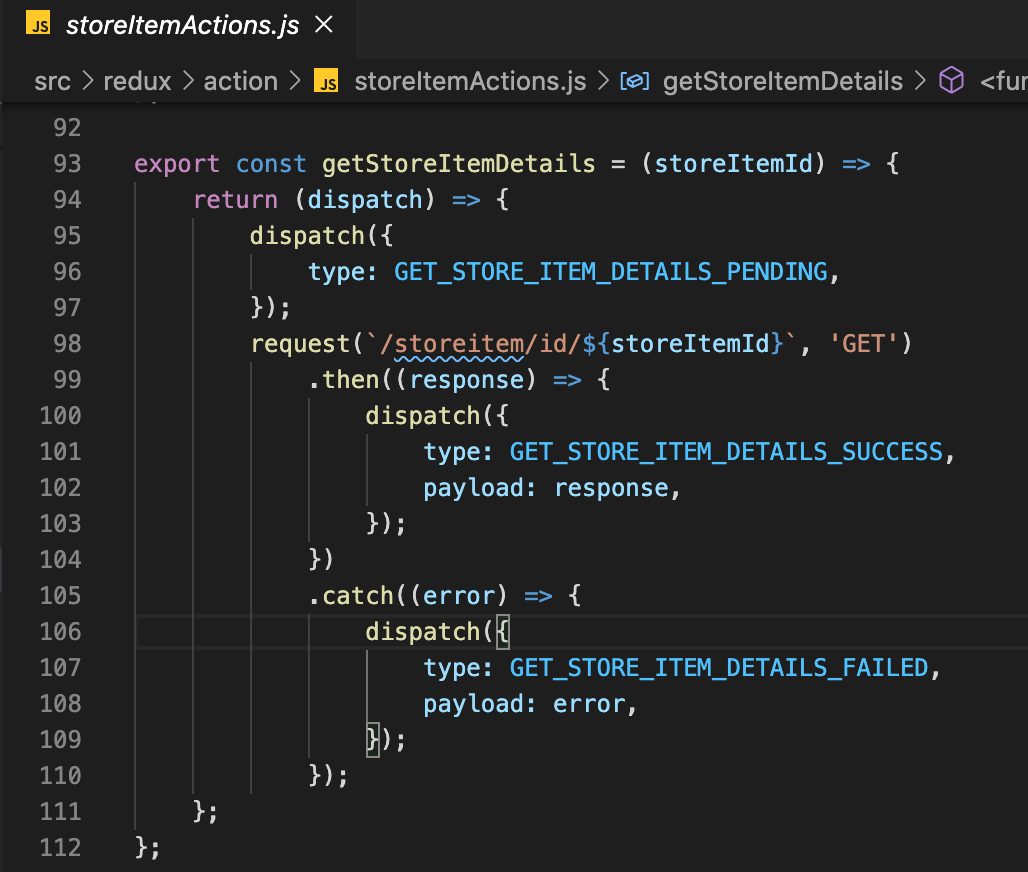
\includegraphics[width=10cm]{./assets/images/actionExample.png}}
\caption{The http request code as an example of abstraction.}
\label{fig:actionExample}
\end{figure}


\subsection{Web Application}
The web application of the system has been written in the React JavaScript framework. The functionality of the application is largely the same as the mobile application however because the web view is available on a larger screen size I have used this to my advantage and included slightly more information for the user. 
The functionality for the web application also differs slightly by offering a different view for managers who are able to view the items and information of other stores as well as their own. 
Figure ~\ref{fig:WebUi} is a screen shot of the application which includes the functionality to change stores.

\begin{figure}[H]
    \centering
    \frame{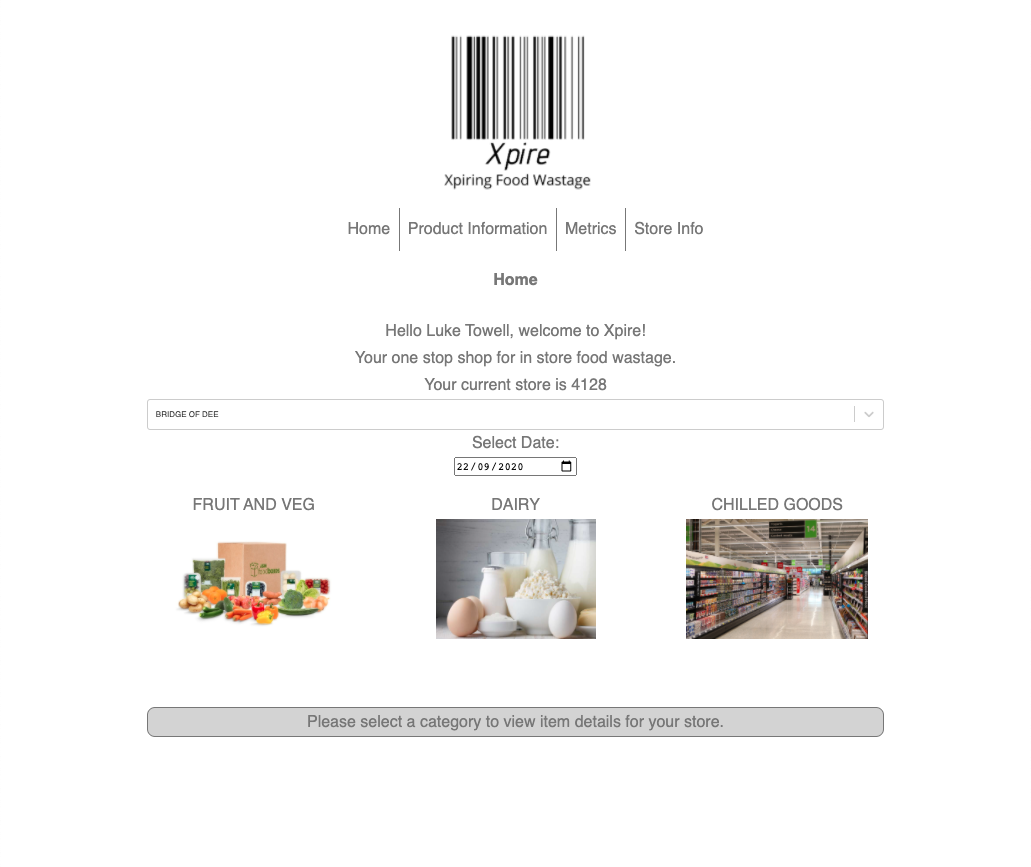
\includegraphics[width=10cm]{./assets/images/webHomeUI.png}}
    \caption{Screenshots of the initial landing page of an authenticated user.}
    \label{fig:WebUi}
\end{figure}

Appendix ~\ref{appendix:webUI} details the screen shots of a users journey through the web application and demonstrates the information that is available to the user.
As was mentioned previously the web application contains some extra functionality which the mobile application does not currently offer.

This functionality includes the ability to query for items which are expiring on specific dates which is chosen by the user on the homepage. This feature allows users to view items which are going to expire in the future or view items which have previously expired and view what actions where taken against them by store colleagues.
other functionality also includes the ability to change stores and view items which are expiring in other stores. 

\section{Web Services}
In order to manage the communication between the front end applications and the database I have written web services in Java using the Spring Boot framework. 
The application has been designed using the "repository pattern" which is discussed in the Gang of Four Book, Design Patterns: Elements of Reusable Object-Oriented Software\cite{gamma1994design} which creates an interface between the front end user and the database. This enables the system to ensure that the data being provided from the front end application matches the expect input and data types that is expected by the database tables. The level of abstraction also allows the developer to manipulate and control the data after is has been retrieved from the database but prior to it being returned to the front end application.

\subsubsection{Documentation of the Web Services}
All of the web services that are available have been documented using the swagger plugin which has enabled me to easily document all of the endpoints that I make use of in the web services. this documentation allows other future developers to easily make use of the web services in their own front end application by providing them with the endpoint URI, the expected parameters and the responses which are provided under certain situations. Appendix ~\ref{appendix:webservices} details how the Swagger UI documentation is displayed and how a developer can make use of the documentation in order to view details about the services and test the relevant services.

\subsubsection{Handling of Environment Variables}
As discussed in the front end applications I have also made use of environment variables in order to manage application configuration values between the different environments. This ensures that the configuration is not hardcoded and can easily be updated or replaced on compile of the web services code. It enables me to easily connect the application to different data sources so that data can be kept separate in other environments for example data in the dev environment does not accidentally make it into the production environment. 


\subsubsection{Deployment of Web Services}
Because the web servers are written in Java you would tradtionally run the web application on a web host e.g. Microsoft Azure or Amazon Web Services (AWS) which would host the web services on an Apache TomCat server. Since this application will be ran in the ASDA environments I have set up the application using docker which allows me to create an docker image which can be ran on a Kubernetes cluster within the ASDA cloud environment. 
By using Docker I am able to run the application in isolation on the Kubernetes cluster and I am also conveniently able to make use of in built monitoring and alerting if there is any issues with the application whilst it is running. 


\section{Testing of the Applications}
Manual Testing
Automated service testing using Swagger and Insomnia.
Ideally would have liked to write both unit tests and end to end tests.

\chapter{Evaluation}
\section {Successes of the project}
Overall based on the aims of the project I believe that the project has been a success. I have produced a system which comprises of several different applications whilst making use of several different programming languages and design concepts. 
 Whilst there have been issues over the course of the project I have received positive feedback from the Project Manager colleagues within ASDA who have been overseeing the project.
I believe that with more time to go through the correct security checks that are mentioned in the challenges section of this report that the project would demonstrate a reduction in 
colleague time spent checking waste stock and an overall increase in colleague performance. 
\\
\\
In the dissertation which will follow this report I plan on going through the individual aspects of the project and identifying how I believe that they have been positively addressed.

\section {Challenges of the Project}
Throughout the project there have been issues which have arisen as the solution has been developed. In the early stages of the project it was identified that due to data security and authentication security utilised by ASDA I would be unable to make use of ASDAs data and authentication systems. This has presented various different issues which include:
\begin{itemize}
    \item Data availability
    \item User Authentication
    \item Application and Database hosting
    \item Store Usage
\end{itemize}

All of these issues have been over come or worked around in order to produce a working software system. Each of the Issues listed above will be discussed in more detail along with the relevant work arounds in the dissertation of this project.


\section{Colleague Feedback}
Unfortunately due to the limitations that have been mentioned above and will be expanded upon in my dissertation I was unable to place the system into a production ASDA store.
Because of this I have had to re-assess how I will gather feedback on the system. The project will now be assessed by ASDA colleagues and managers based on demonstrations of the application within different user scenarios. 
In my dissertation I will discuss the feedback which I receive and summarise the positives and potential improvements that the ASDA colleagues raise in their feedback.

% Add in feedback and critical analysis of feedback from Philippa and Holly. Must be anonymous. talk about current implementation and differences between solution developed.
% talk about functionality that is positive and the feedback given
% talk about improvements that are raised and relate them to the potential future works. 

\chapter{Learning Points}
Over the period of the project several technologies have been used within the software system
which I have either used in a limited capacity or I have not used at all. In this chapter I will
detail which technologies I have had to learn in order to complete the project, which skills and 
technologies I will make use of again in the future and what I will avoid the next time I have to 
complete a similar project.

% Java Spring Boot
\section{Java}
The web services are a central part of the system. I decided that in order to write a truly scalable
and enterprise worthy application I would write the RESTful web services in Java using the Spring Boot framework.
\\
\\
I chose Spring Boot based on the fact that it a widely adopted java framework which is already utilised
within the ASDA / Wal-Mart ecosystem. I have previously worked on applications which make use of spring
boot however I have never initialised an application or written an entire suite or RESTful services.
\\
\\
Spring Boot was an interesting framework to work with as there was plenty of documentation available online,
the process of initialising the application was straightforward using the Spring Boot Initializr TODO:insert reference to Initializr. 
Spring Boot is an opinionated object orientated framework which is very different to my typical background 
of JavaScript Node applications. In order to efficiently make use of Spring Boot I have had to learn the nuances
of the framework such as how to architect and organise the application structure as well as 
researching the various design patterns to use when creating the application. 
\\
\\
After thorough research into object orientated design patterns I decided that because I was integrating my endpoints
with a SQL database the best design pattern for the application would be the "Repository Pattern". This is because 
via using the repository pattern the query logic for retrieving databases was easily abstracted out from the other 
application code. It also ensures that the objects which are being submitted to the services and written to the database
match the format that the database is expecting.
\\
\\

Overall I would say that the use of Java Spring Boot was really beneficial to the project and my own personal development. I have furthered 
my knowledge of creating RESTful services and object orientated programming. The use of Spring Boot has forced me to look into development 
principles and design patterns that I haven't previously been exposed to which will improve my knowledge of software engineer and improve 
the quality of the applications that I write in the future.


% SQL and Database integrations
\section{Database Implementation}
In other applications I have made use of SQL databases however normally these databases have been designed and created by other qualified data architects.
Throughout this project I have designed and implemented my database structure which has presented me with several opportunities to further my knowledge.
I have needed to research how to efficiently design a database in order to reduce duplication of data and to ensure that the data was easily queryable by the applications. 
One of the main learning points which I had no previous experience was the creation of foreign keys and table relationships.
In order to successfully create an efficient database I have had to research and consider how each table is related to each other 
and how I would be able to effectively store applicable data in the database.
In order to design an effective database structure I looked into documentation online as well as making use of online platforms
to assist with a visual DB schema which assisted me by presenting a visual diagram which was easier to understand.

I believe that the process which I have completed in order to design and implement the SWL database within this project
has assisted in developing my data management and database creation skills. 
I will be able to take the techniques and knowledge that I have learnt whilst working with the data in this application
onto other applications which I work on in the future. 


\section{Project Skills}
As well as the above technical skills, this project has been an excellent opportunity to improve on my professional skills.
Over the course of the project I have been involved with organising various meetings, communicating with professionals within the ASDA business and the University of Liverpool as well as ensuring that the project was completed within the time scales that were outlined.

I have had to ensure that my organisation, time management and project management skills have been as professional as they could be in order to achieve all of the tasks listed above. 
Whilst there is not a measure or metric which can indicate how successful I have been in making use of these soft skills I am confident that the project has improved my skills and provided me with the confidence to carry forward the various skills onto future projects that I am apart of.

\chapter{Professional Considerations}

In this chapter I have Considered each of the 4 main principles outlined in the BCS code of conduct and I have detailed how they have been considered and met throughout the project. 

\section{Making IT for everyone}
The project was focused on the production of a software system which can be accessed by multiple colleagues from multiple devices across the asda store estate.
 With this in mind design and usability was a key focus of the project to ensure that the system was easy to use and simple to understand. 
 \\
 \\
 As can be seen in figure TODO:(insert link to designs) and is discussed in the design chapter of this dissertation the applications have deliberately been kept simple and minimalistic to ensure that the user is not overwhelmed with unnecessary information.
  I believe that this approach has enabled me to develop a system which specifically calls out to the standard of making IT for everyone by promoting equal access to the application and therefor equal access to the benefits that the application offers. 
\section{Show what you know, learn what you don't}
This project has been produced solely by myself and all work on the applications has been written and architected by the author. 

Whilst working through the project there have been various skills / languages that I have not been familiar with which I have had
to research and learn whilst developing the applications which form part of the system. The skills which I have had to focus on include
creating writing applications written in Java which is a language I have had very little previous experience with and the creation and architecture of a SQL based Database.
These points have previously been discussed in more detail in chapter 7 however I feel like they are an excellent example of how 
I have developed my professional knowledge of two technologies in order to complete the project.
\\
\\
I have also attempted to "Learn what I don't know" through the use of feedback gathered from employees and academics 
in order to identify potential improvements which could be incorporated into my application. 
This has involved the use of professional meetings and discussions which are further discussed in Chapter 6.


\section{Respect the organisation or individual you work for}
Due to the fact that this software system has been created for the use of a large national retailer it was essential that the produced system is in tune with the organisations values and principles. 
As part of ensureing respect for the organisation that I work for I have diligently ensured that any functionality which I was unable to expose for security reasons this has included the authentication of the application as well as the data structures which are used internally has been mocked out.

I have maintained respectful and purposeful communication using regular meetings with the project management and professional resource provided by ASDA to ensure that the project was on track and was meeting the requirements that where outlined initially.

Finally I completely accept all responsibility for the software system that has been produced as part of this project. 

\section{Keep IT real, Keep IT professional. Pass IT on}
Throughout the development of the software system produced in this project I believe I have represented the BCS principle of 
"Keep IT real, Keep IT professional. Pass IT on" by ensuring that I have remained professional in all communications between
myself and others involved in the project. I have ensured that any knowledge that I have learned is well documented in order
to be easily passed onto other software engineers and In summary I believe that the project has improved my personal professional
standards and development abilities.

\chapter{Conclusions}
% How do I feel the application has been completed?
\section{Personal Conclusion}
% What would it take to put the application into production
\section{Productionisation}
% What extra work could be completed in order to finish the application?

\section{Potential Expansions}
% Potential for project expansions?

\subsection{Timesheeting}
Through the use of data mining from the data collected by the application, we should be able to accurately predict
how long it takes staff to organise and mark down the expiring items within their respective departments. Once 
this data has been collected then theoretically it could be used in order to calculate how many staff are needed 
in order to mark down items on a particular day depending on the number of items that need to be reduced as well 
as the length of time that it is likely to take the staff in order to mark down or redistribute the expiring stock
on the shop floor. 

\subsection{Stock Prediction and Inventory Management}

By analysing the number of items which are expiring in individual stores we should also be able to perform trend 
analysis on the data which should highlight items of stock which are repeatedly marked down. This trend analysis 
could then be used to inform store managers and the ASDA inventory management systems of any over ordering which is 
occuring and allow for more accurate stock levels to reduce potential waste in the future.

\subsection{Item Location}

\subsection{Item Prioritisation}
%%%%   REFERENCES

%%%%  Section for references, using the \bibitem directive to 
%%%%  specify labels used to cite sources in the document.  

\addcontentsline{toc}{chapter}{Bibliography}
\bibliography{bibliography}
\bibliographystyle{plain}


%%%%   APPENDICES
\newpage
\addcontentsline{toc}{chapter}{Appendices}
\begin{appendix}
    \chapter{User Interface Designs}
    \section{Mobile Designs}
    \label{appendix:mobileDesign}
        \begin{figure}[H]
            \centering
            \frame{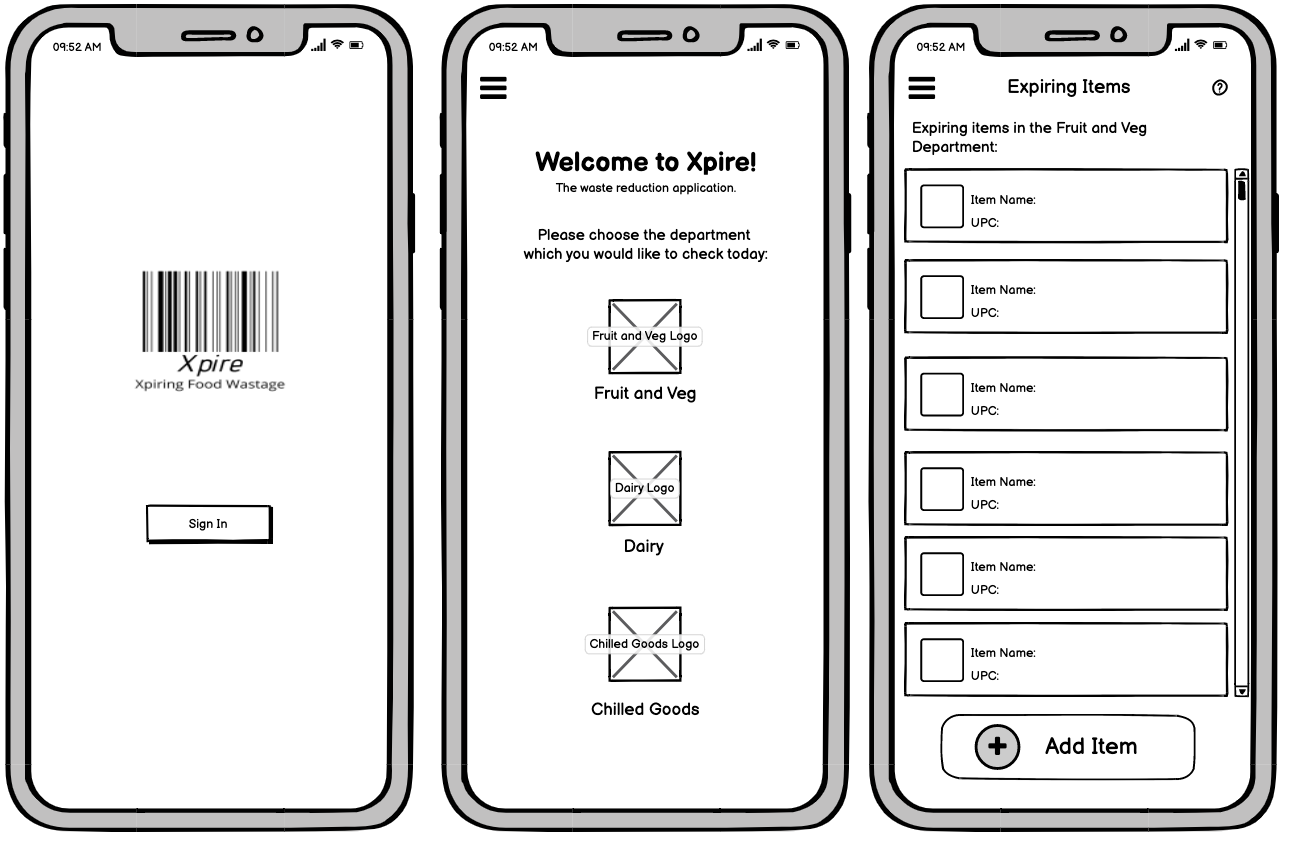
\includegraphics[width=9.5cm]{./assets/images/mobileUIpt1.png}}
            \caption{The mobile application user interface designs, including the Login, Category list and Item list screens from left to right.}
            \label{fig:mobileUIpt1}
        \end{figure}
        \begin{figure}[H]
            \centering
            \frame{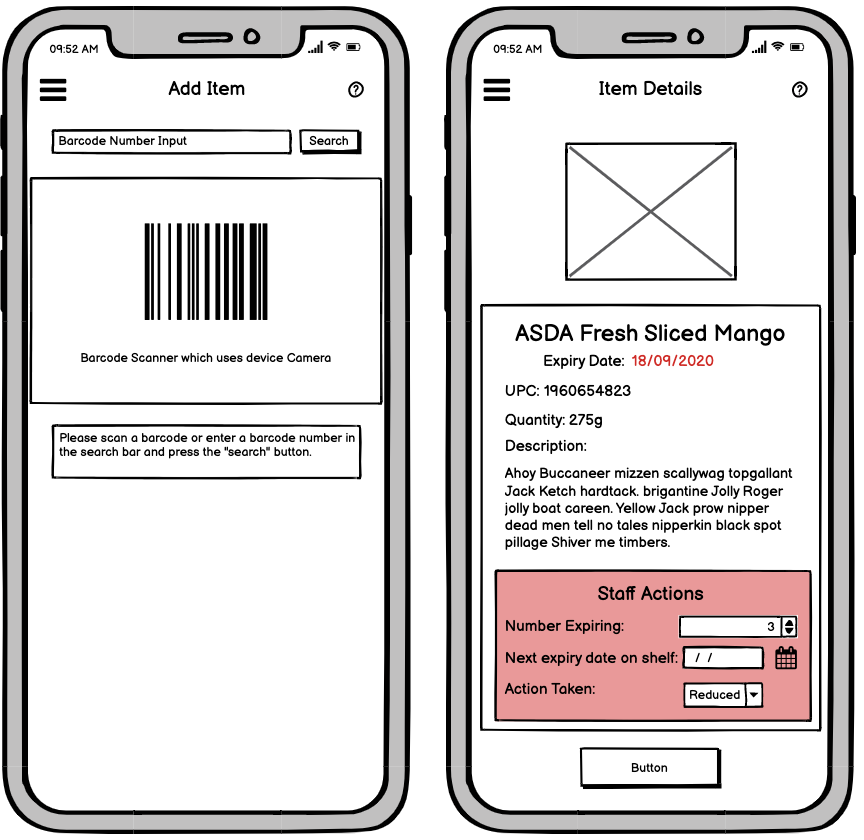
\includegraphics[width=7cm]{./assets/images/mobileUIpt2.png}}
            \caption{The mobile application user interface designs, including the Scanner and Item details screens from left to right.}
            \label{fig:mobileUIpt2}
        \end{figure}

    \section{Web Application Designs}
    \label{appendix:webDesign}
        \begin{figure}[H]
            \centering
            \frame{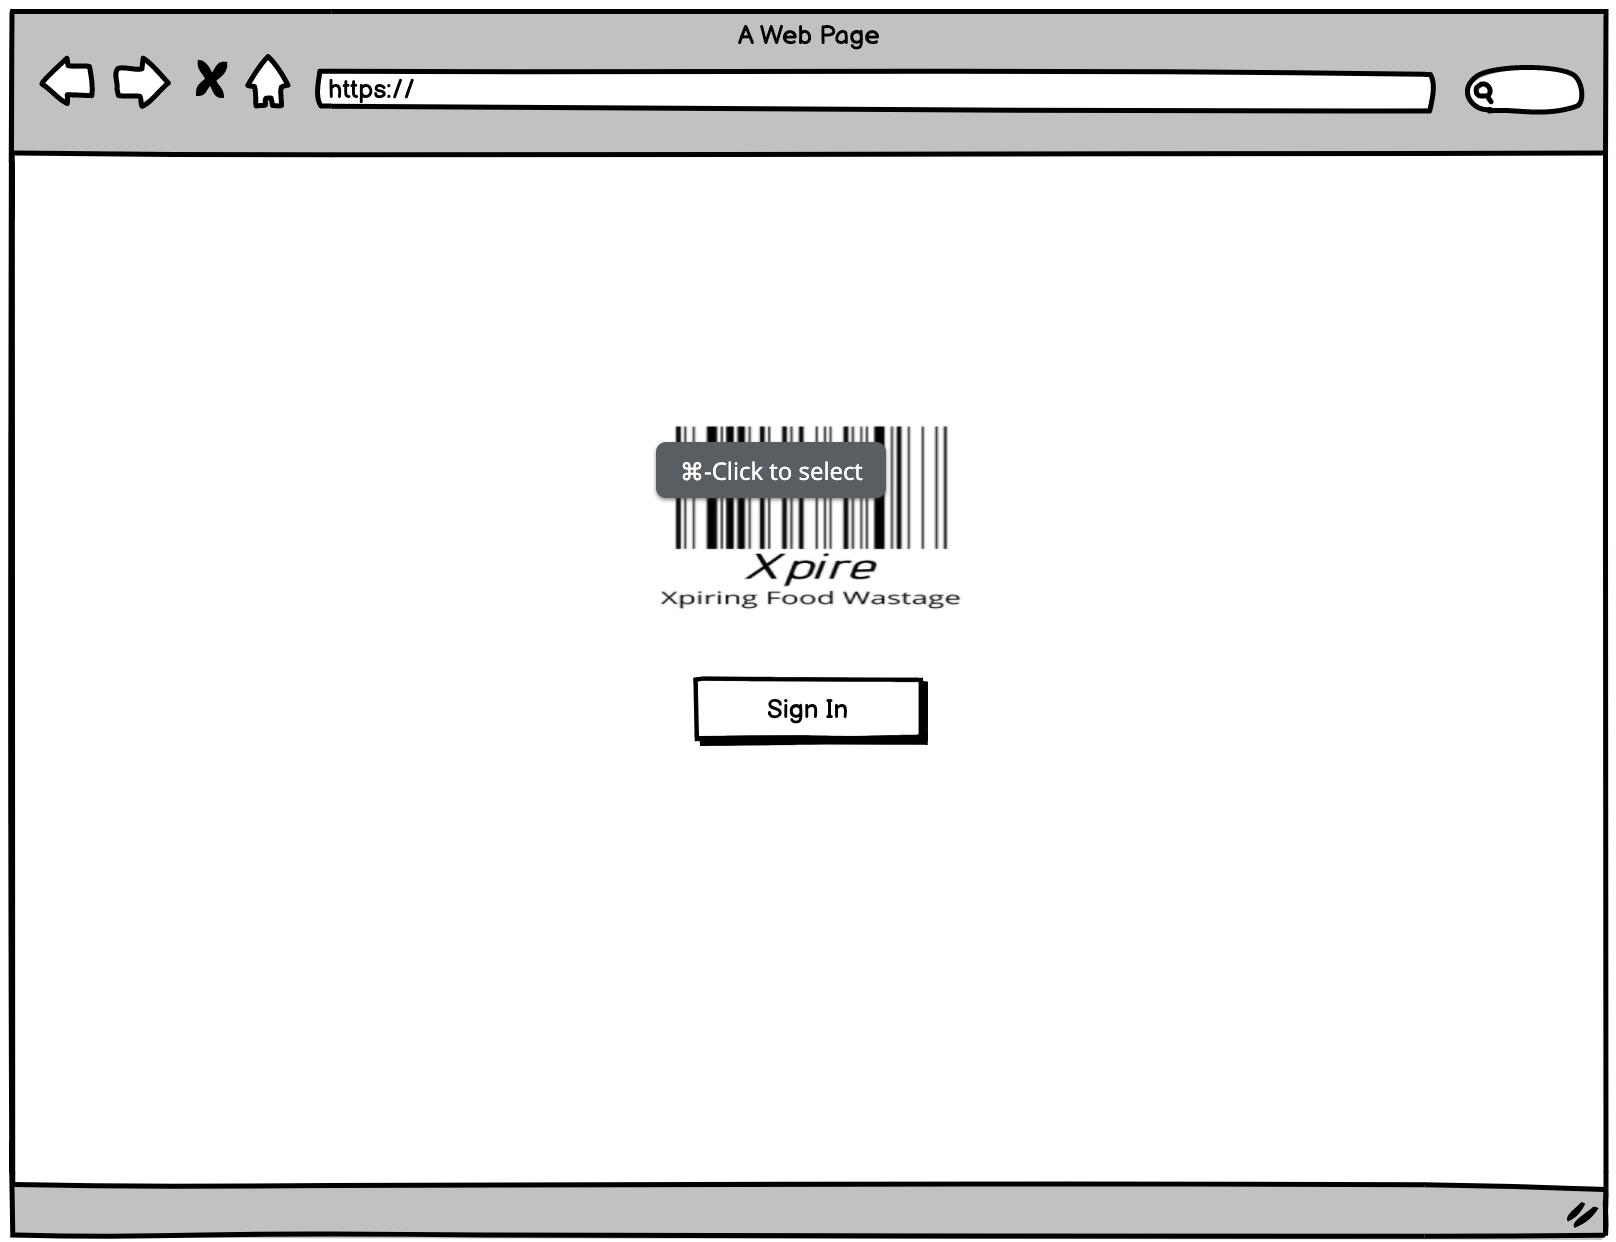
\includegraphics[width=10cm]{./assets/images/webLogin.png}}
            \caption{The design for the web application login screen}
            \label{fig:mobileUIpt2}
        \end{figure}
        \begin{figure}[H]
            \centering
            \frame{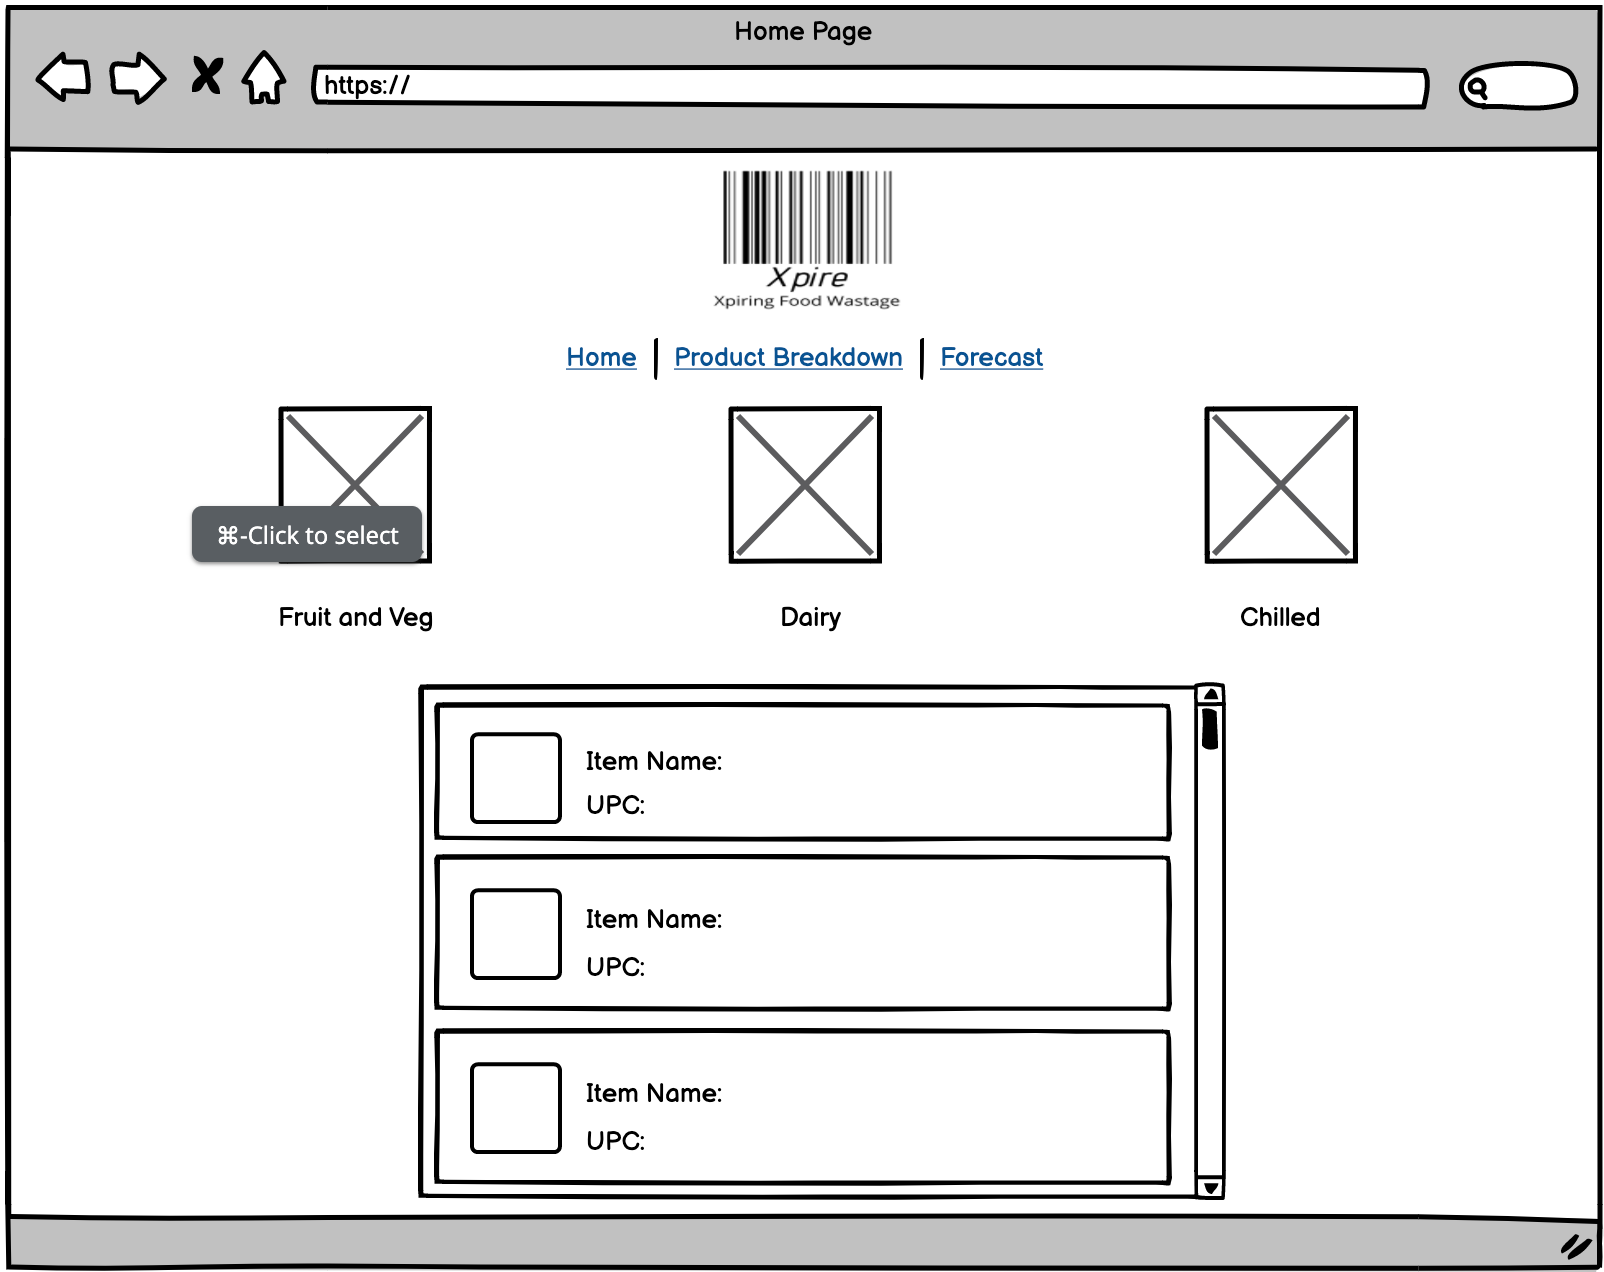
\includegraphics[width=10cm]{./assets/images/webHome.png}}
            \caption{The design for the web application home screen once a user has been authenticated}
            \label{fig:mobileUIpt2}
        \end{figure}
        \begin{figure}[H]
            \centering
            \frame{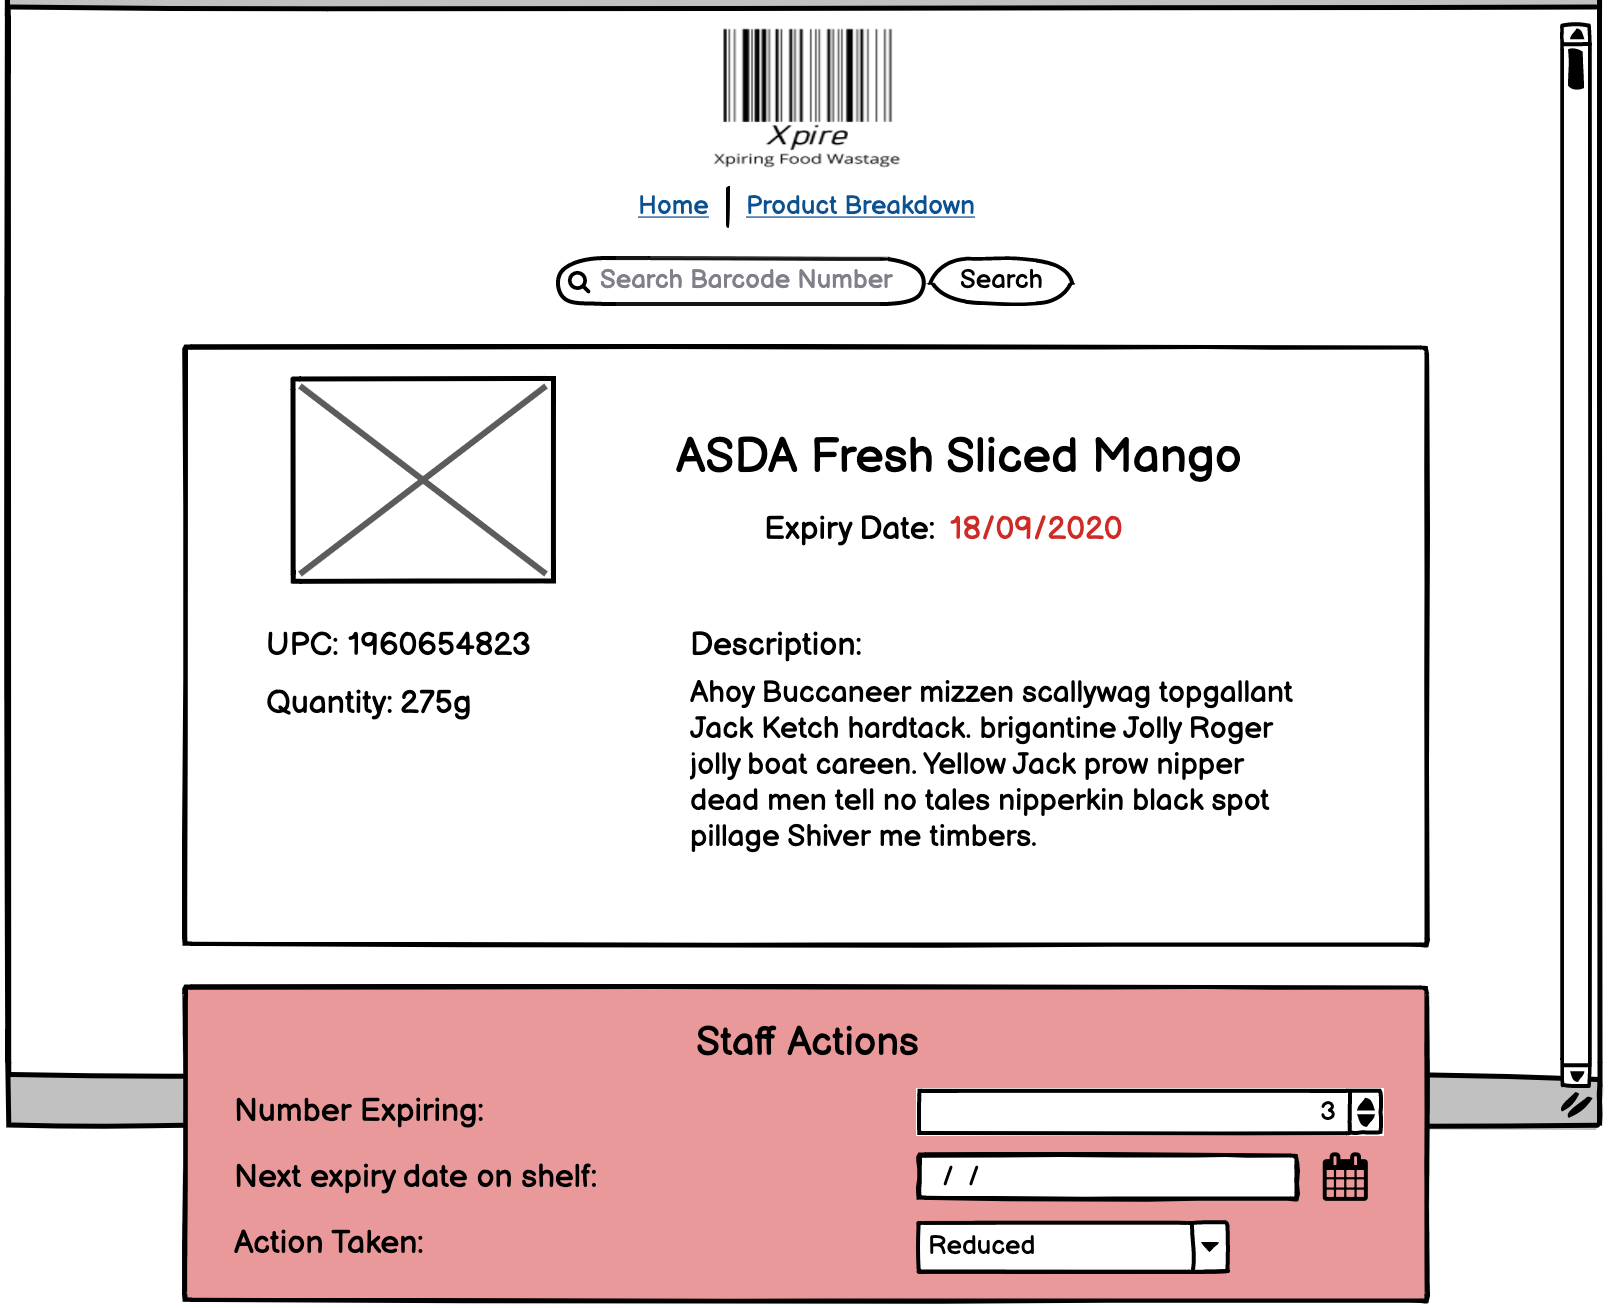
\includegraphics[width=10cm]{./assets/images/webItemDesc.png}}
            \caption{The design for the web application item description screen. This screen is used to display item information specific for the users store.}
            \label{fig:mobileUIpt2}
        \end{figure}
        \begin{figure}[H]
            \centering
            \frame{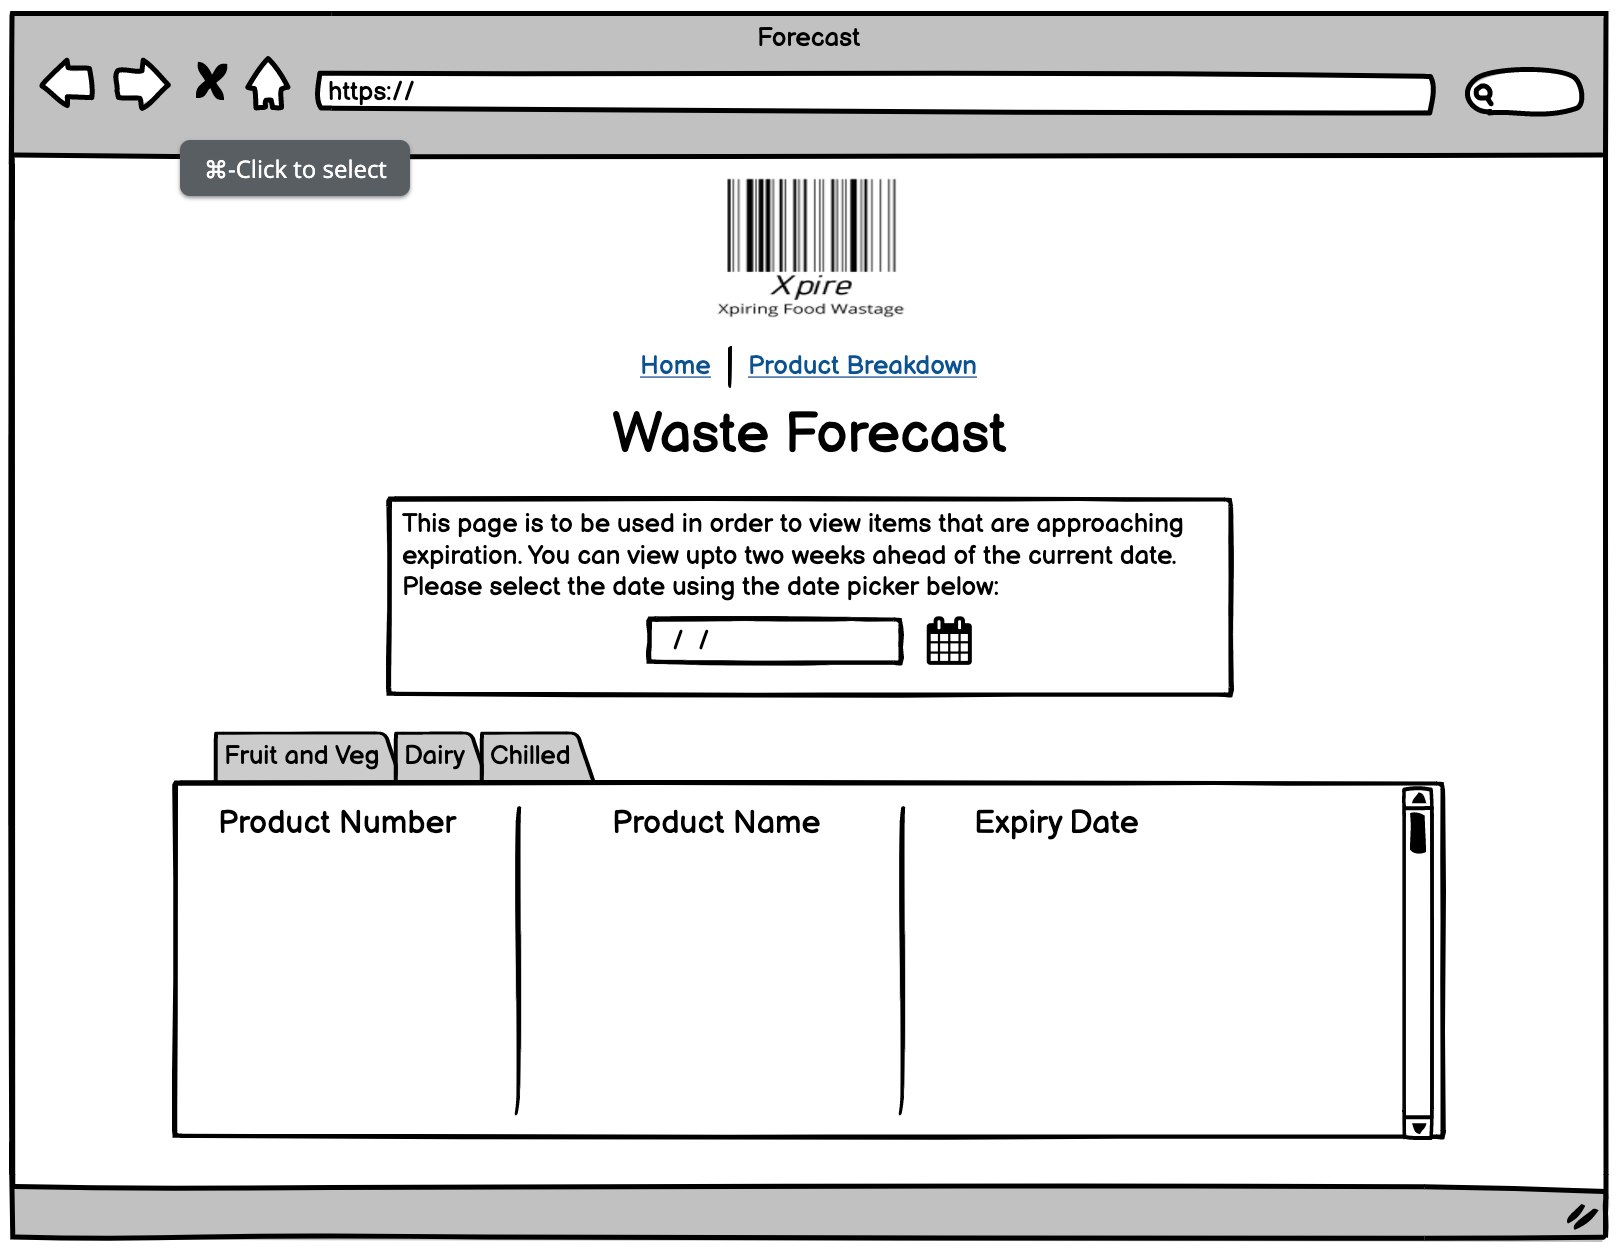
\includegraphics[width=10cm]{./assets/images/webWaste.png}}
            \caption{The design for the web application waste screen. This is a conceptual design for the a waste page which would allow the store manager to view an item based waste summary for their store.}
            \label{fig:mobileUIpt2}
        \end{figure}
        \begin{figure}[H]
            \centering
            \frame{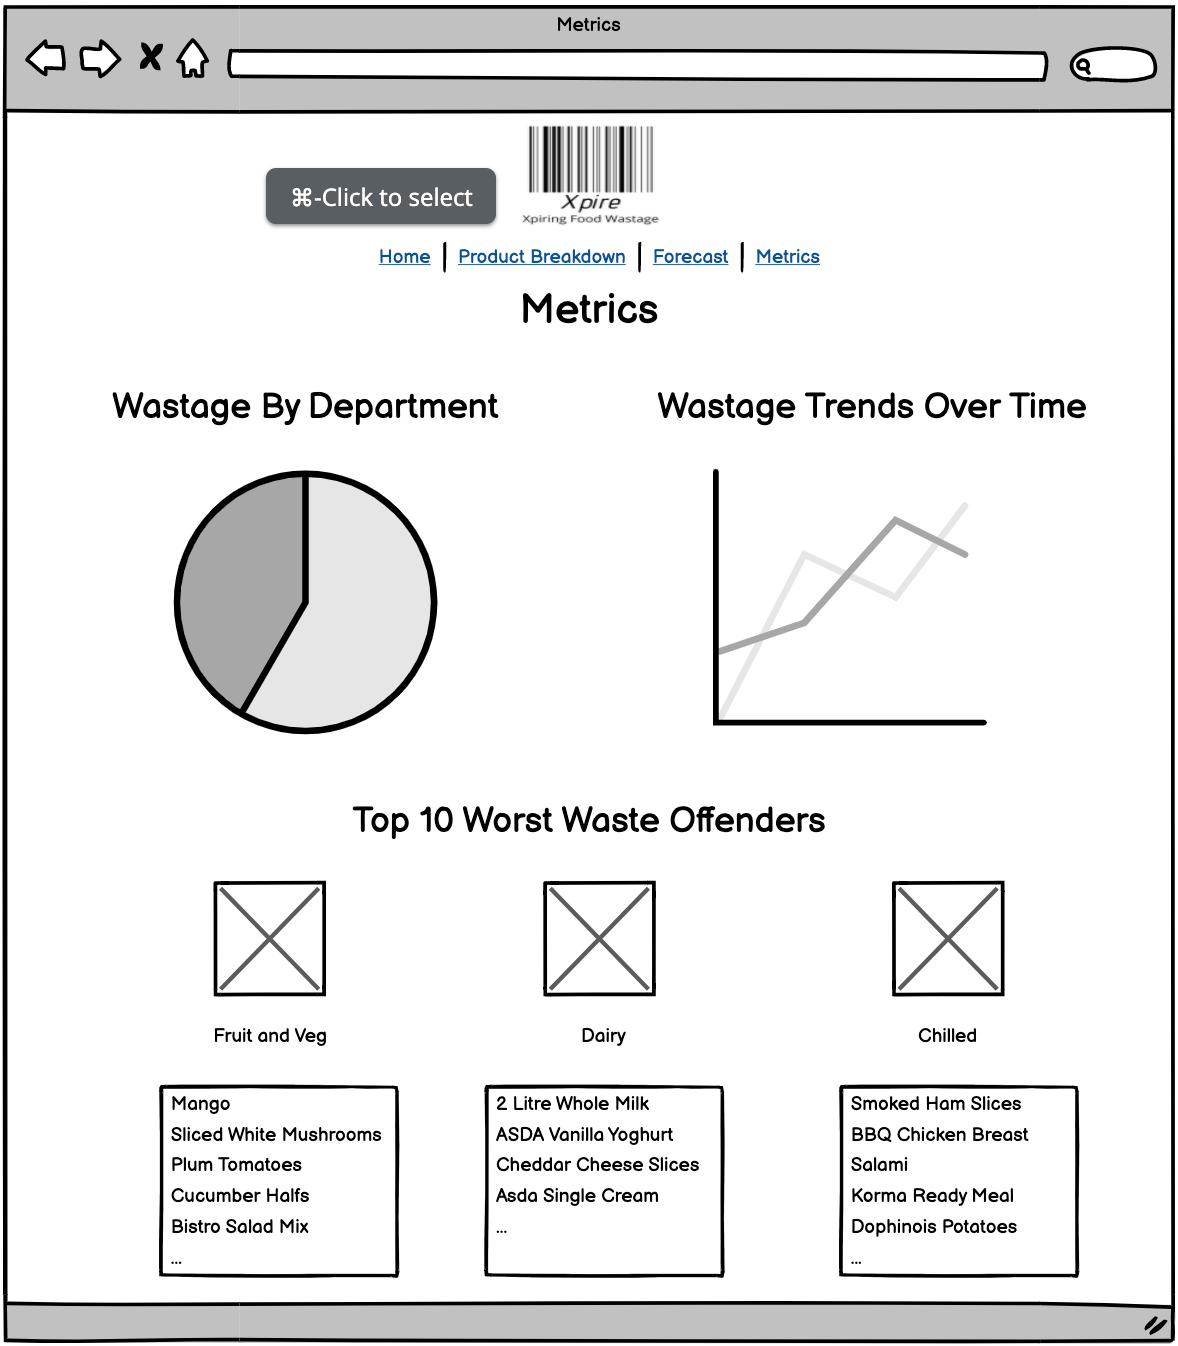
\includegraphics[width=10cm]{./assets/images/webMetrics.png}}
            \caption{The design for the web application metrics screen. This is a conceptual design for the a metrics page which would allow the store managers to view an store based metrics for their store and the items that are often wasted.}
            \label{fig:mobileUIpt2}
        \end{figure}

    \chapter{Database Schema}
    \label{appendix:DBSchema}
        \begin{figure}[H]
            \centering
            \frame{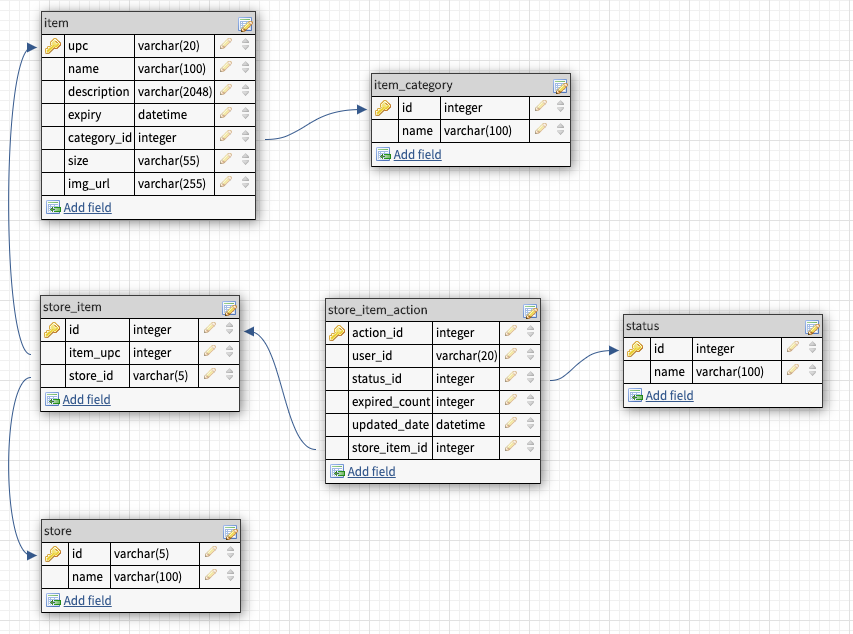
\includegraphics[width=15cm]{./assets/images/Database-Schema.png}}
            \caption{The database schema for the final state of the Xpire database, this schema details all of the tables, columns and relationships.}
            \label{fig:mobileUIpt2}
        \end{figure}
     
    \chapter{Mobile Application User Scenarios}
    \label{appendix:mobileUI}
    
    \begin{sidewaysfigure}[ht]
        \frame{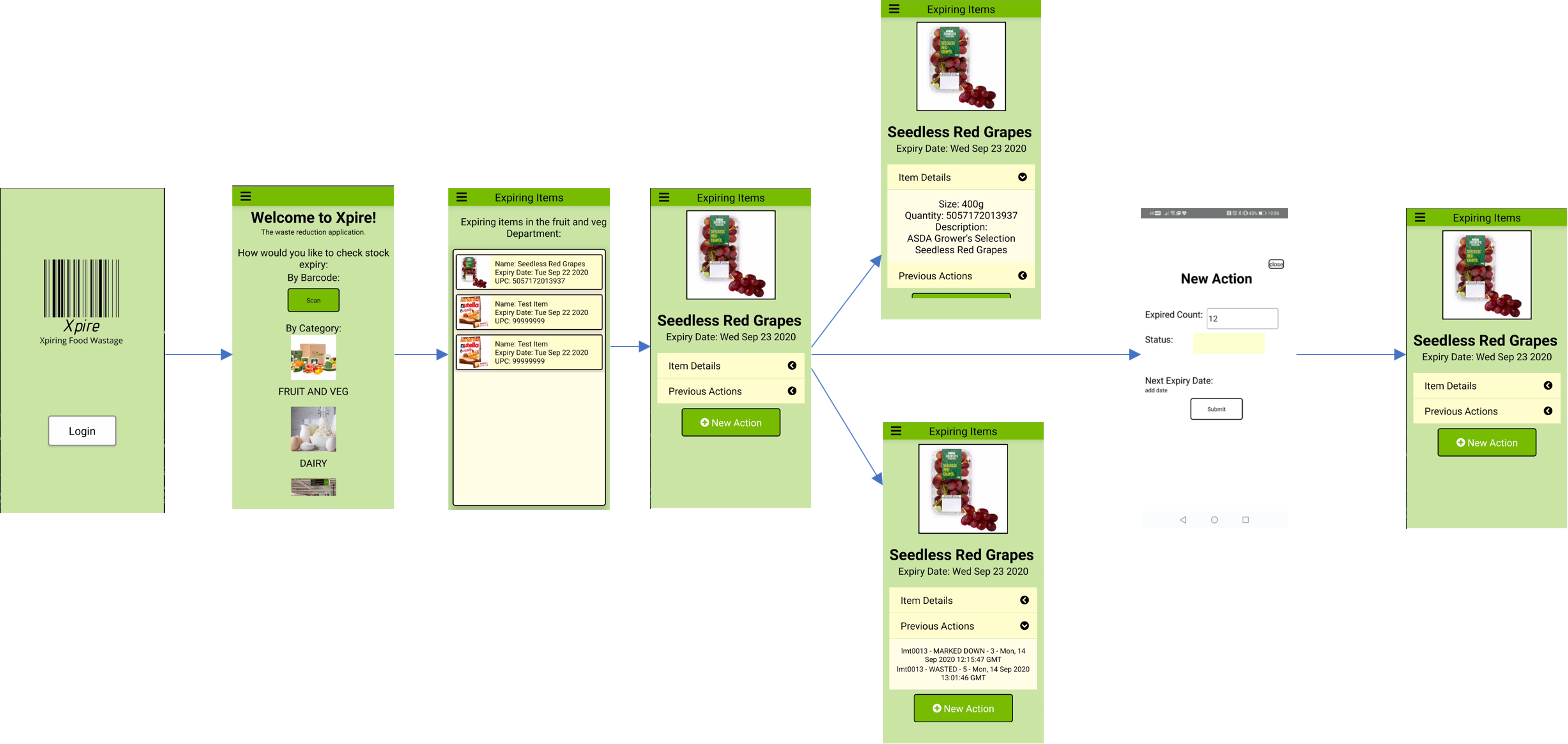
\includegraphics[width=25cm]{./assets/images/Scenario_1.png}}
        \caption{The mobile application and the potential flow a user may take when manually checking category items via the application.}
        \label{fig:mobileUIpt2}
    \end{sidewaysfigure}

    \begin{sidewaysfigure}[ht]
        \frame{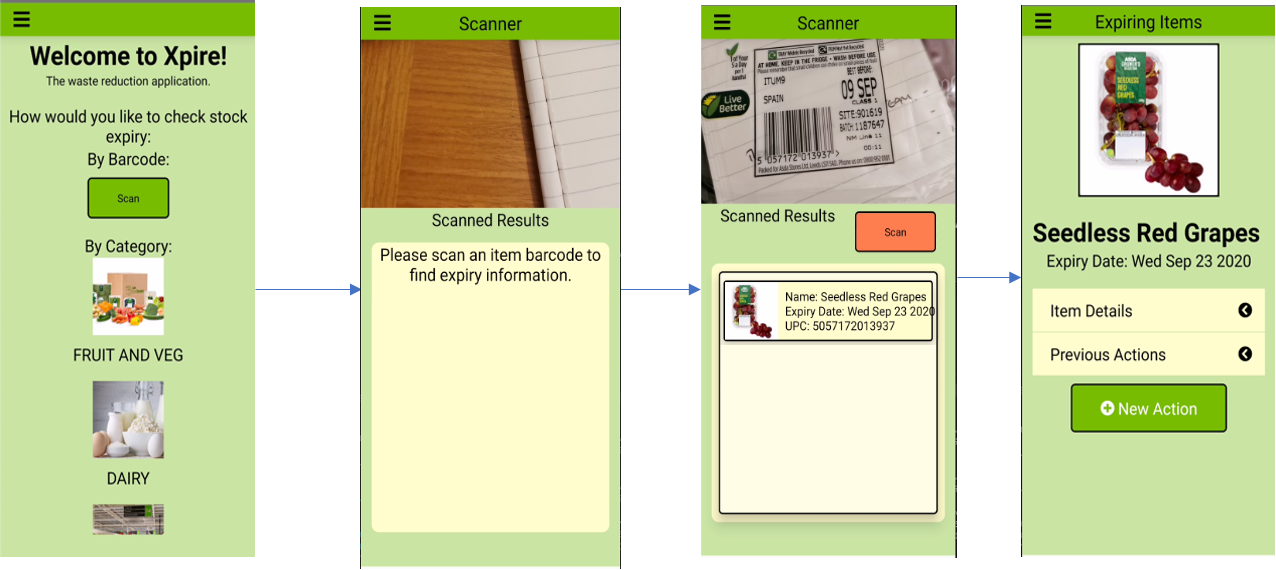
\includegraphics[width=25cm]{./assets/images/Scenario_2.png}}
        \caption{The mobile application usage flow when a user uses the application scanner functionality in order to look up item information using the items barcode.}
        \label{fig:mobileUIpt2}
    \end{sidewaysfigure}
    % this should include the scenario of user logs in and uses category to see which items are going out of date today and then can add actions and view details and previously taken actions
    % Scenario 2 - user scans item to find all expiring items with same barcode. can see items taken on items expiring on different dates.
    % scenario 3 - Expiring item is found in store but not known in app

    \begin{sidewaysfigure}[ht]
        \frame{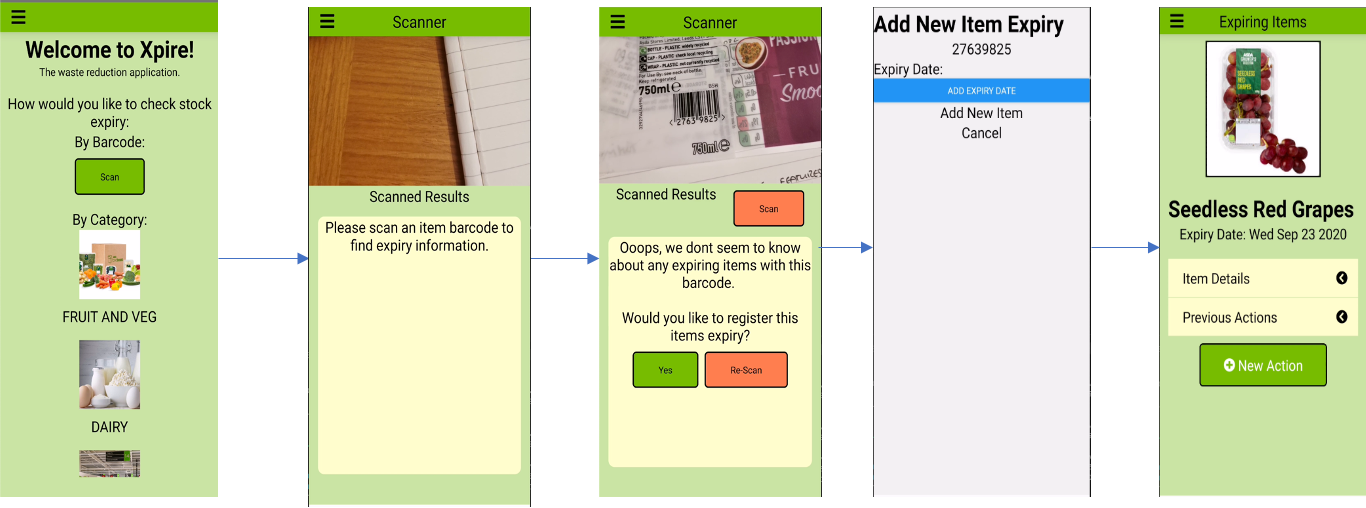
\includegraphics[width=25cm]{./assets/images/Scenario_3.png}}
        \caption{The mobile application usage flow when a user uses the application scanner functionality in order to enter the details for an item in the store which is unknown to the application.}
        \label{fig:mobileUIpt2}
    \end{sidewaysfigure}


    \chapter{Web Application User Interface}
    \label{appendix:webUI}
    \begin{figure}[H]
        \centering
        \frame{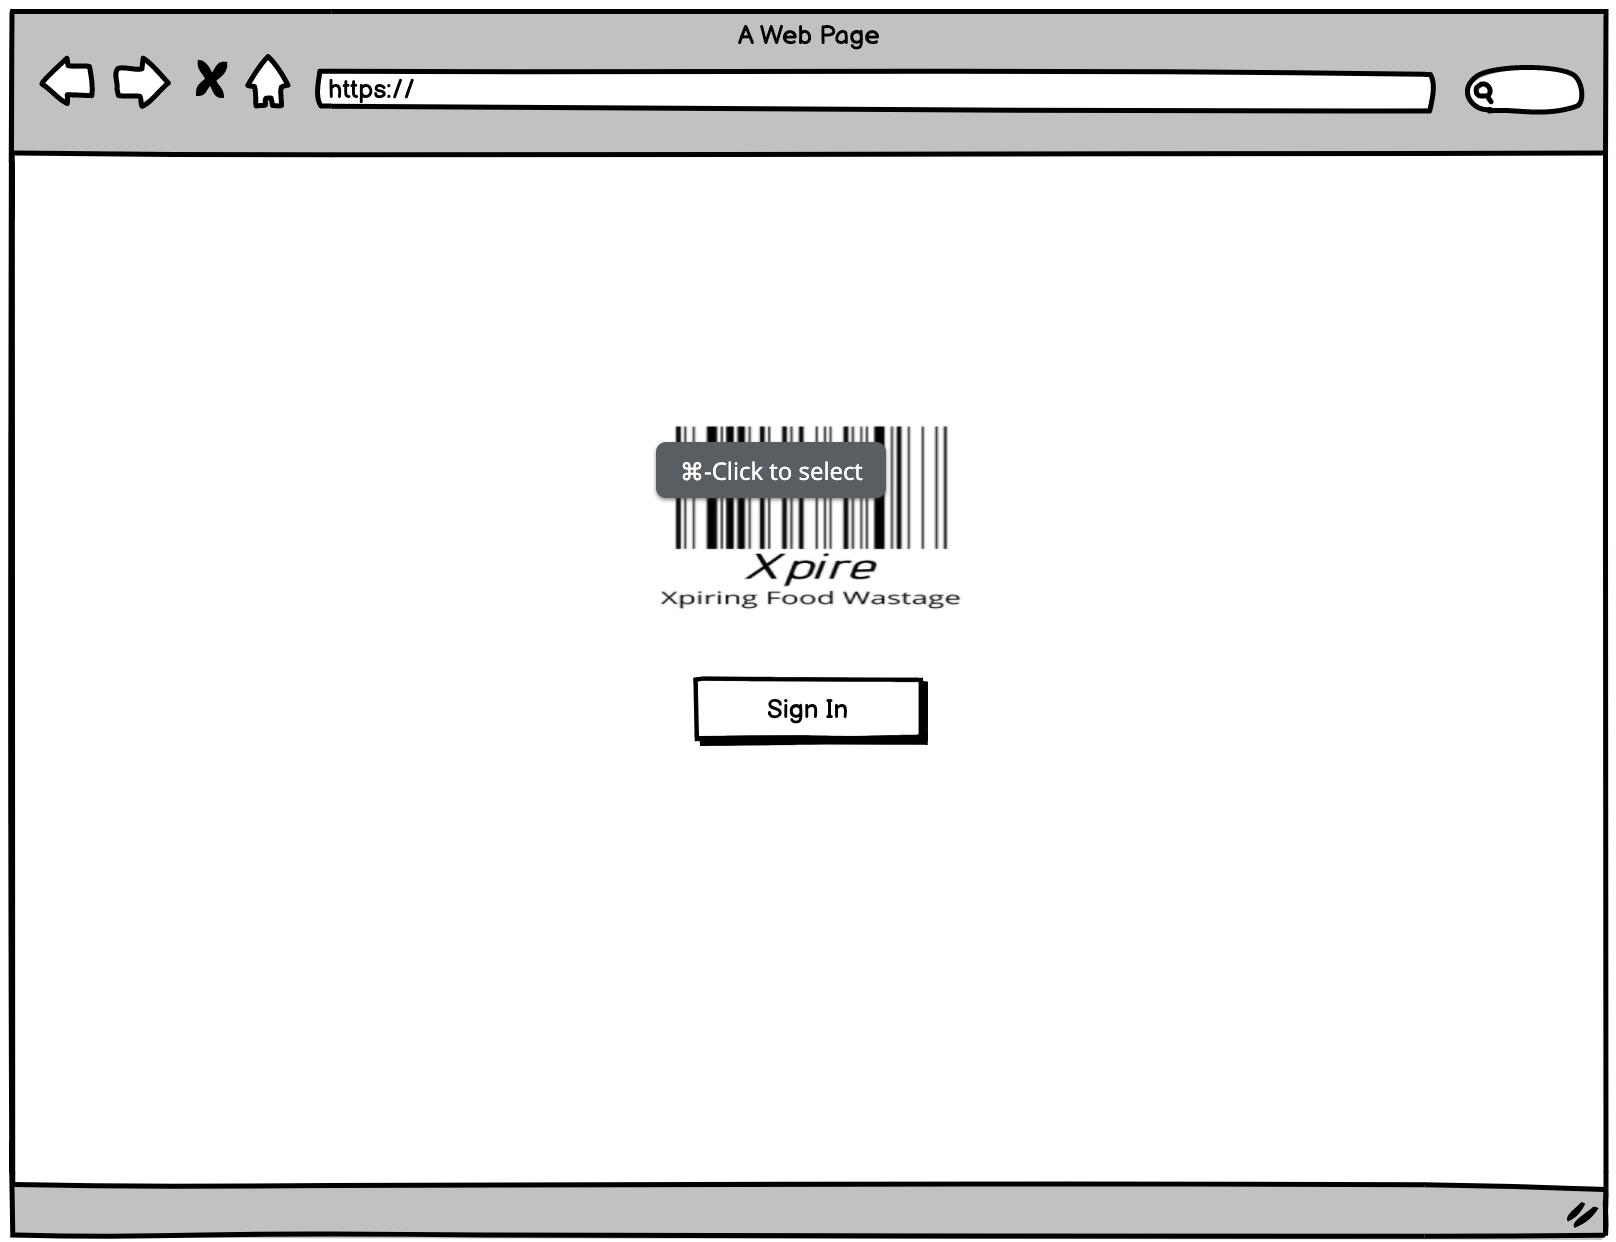
\includegraphics[width=9cm]{./assets/images/webLogin.png}}
        \caption{The web application login screen.}
        \label{fig:swaggerList}
    \end{figure}
    \begin{figure}[H]
        \centering
        \frame{\includegraphics[width=9cm]{./assets/images/webHomeUi.png}}
        \caption{The web application home screen. This page enables the manager to change store, view category and item information for specific dates.}
        \label{fig:endpointDocs}
    \end{figure}
    \begin{figure}[H]
        \centering
        \frame{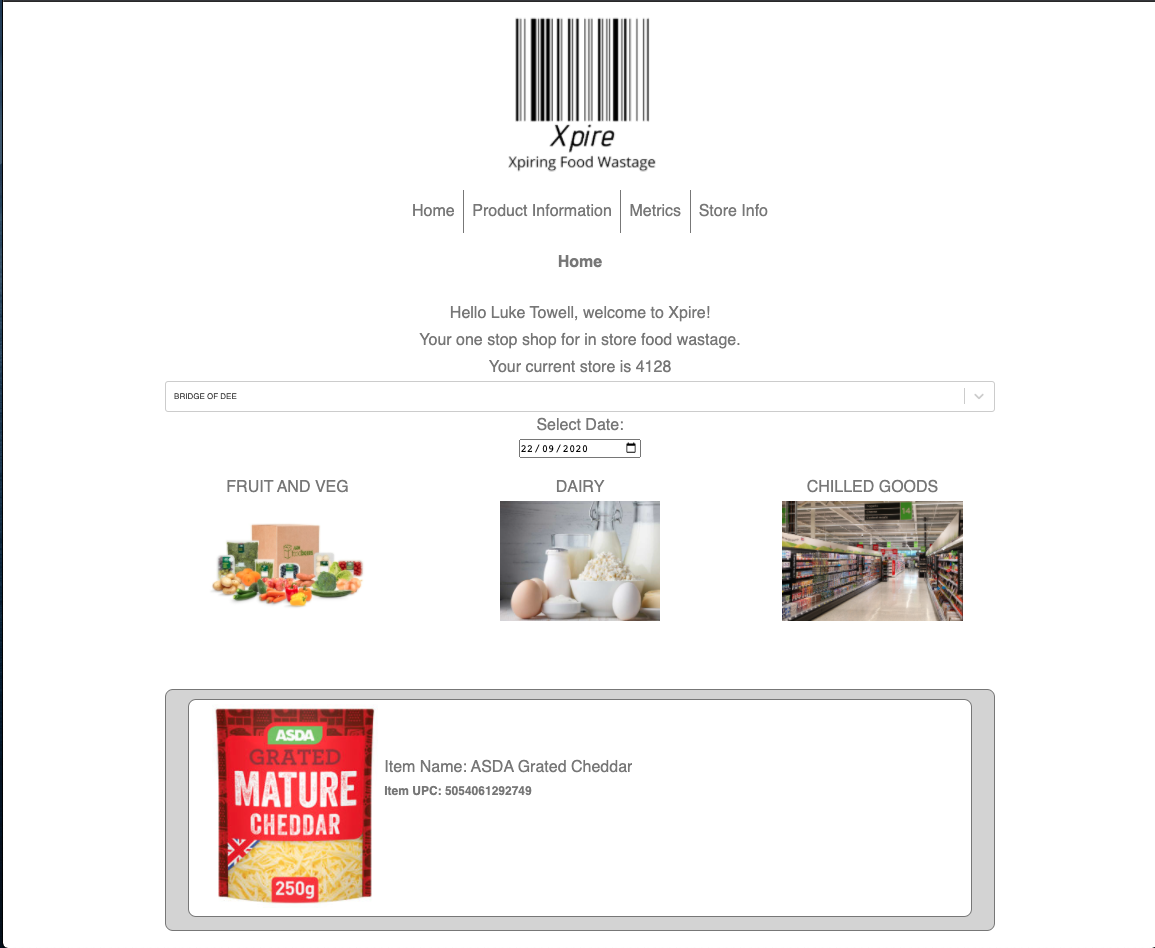
\includegraphics[width=10cm]{./assets/images/webDairyCat.png}}
        \caption{An example of an item being displayed in the home page for the Dairy category.}
        \label{fig:endpointExample}
    \end{figure}
    \begin{figure}[H]
        \centering
        \frame{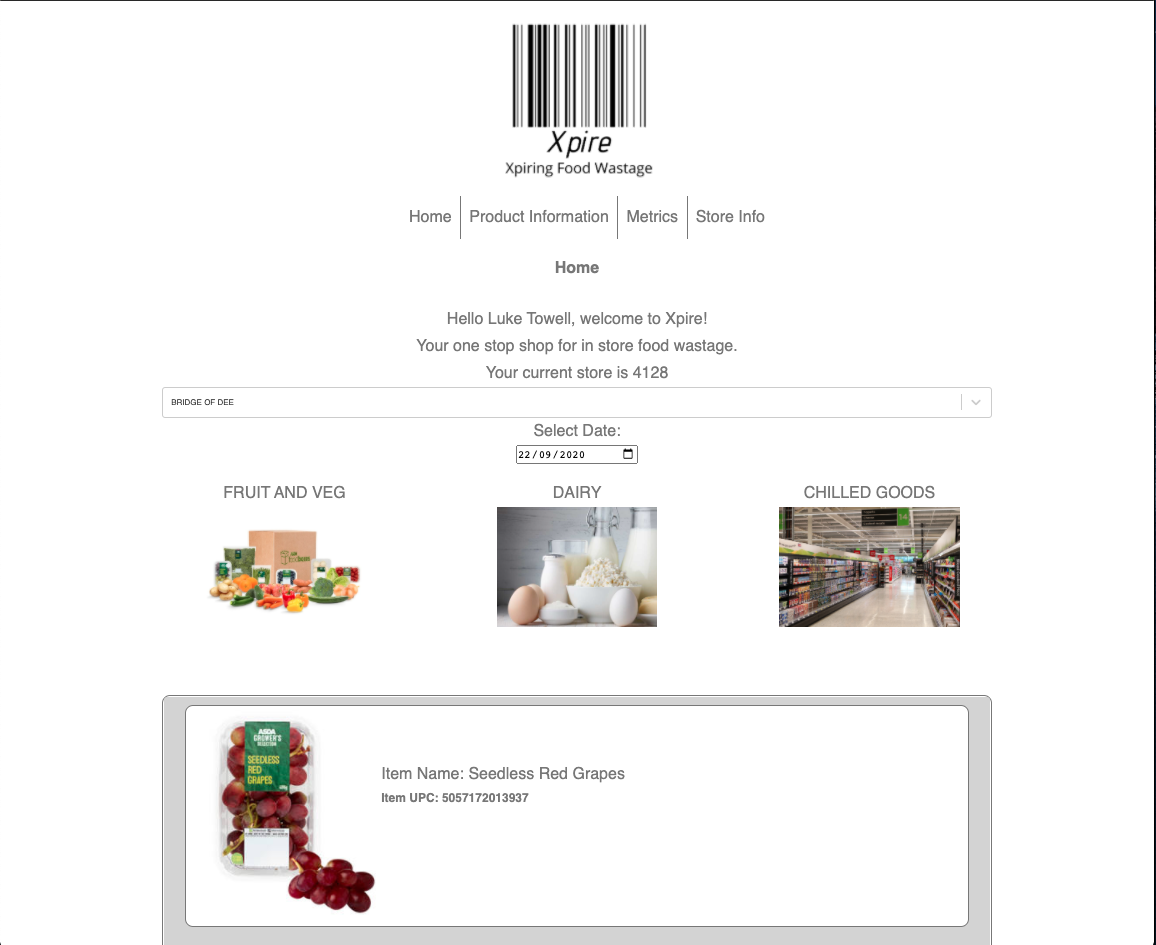
\includegraphics[width=10cm]{./assets/images/webFruitItem.png}}
        \caption{An example of an item being displayed in the home page for the Fruit and Veg category.}
        \label{fig:endpointTest}
    \end{figure}
    \begin{figure}[H]
        \centering
        \frame{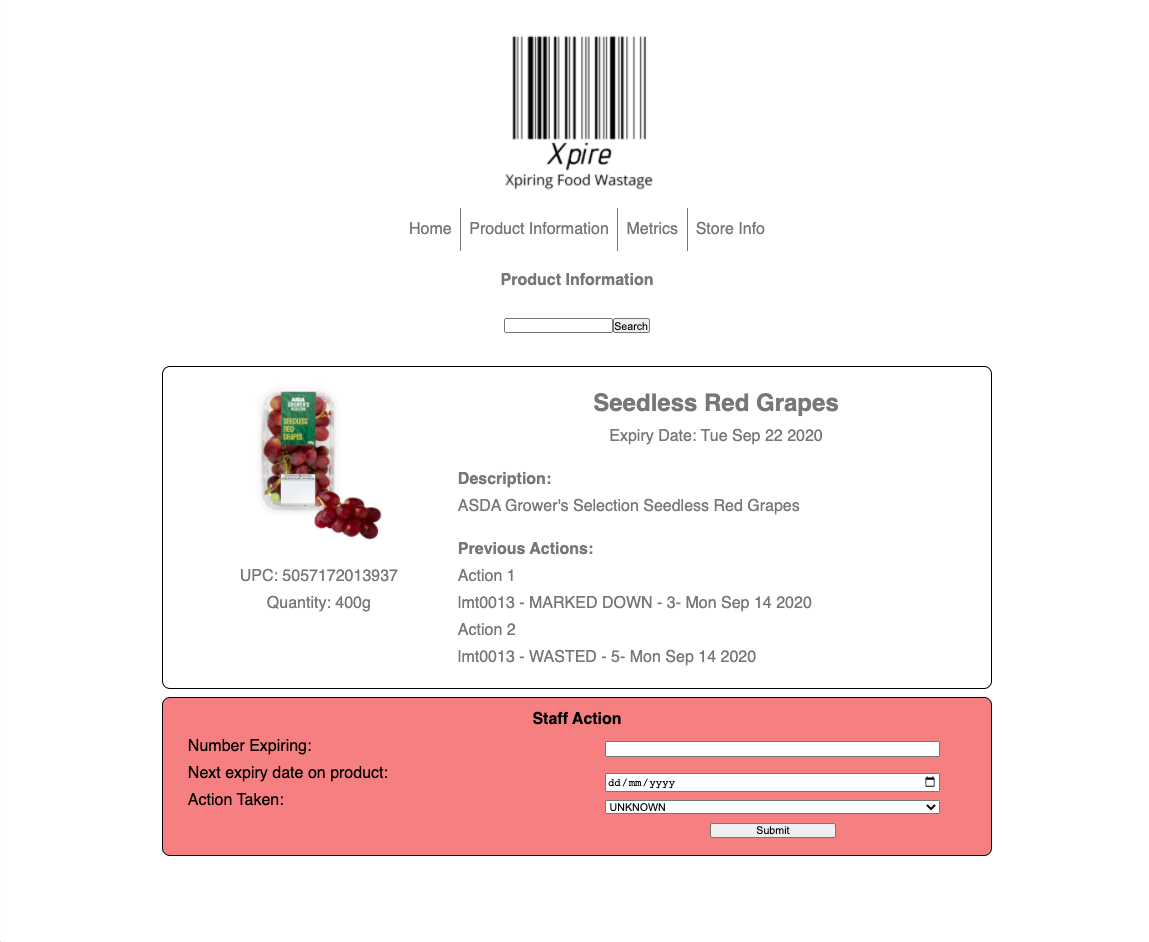
\includegraphics[width=10cm]{./assets/images/webItemDetail.png}}
        \caption{The web application item detail screen. This screen displays all item information to the user. The user is also able to update the item with a new action which they have taken.}
        \label{fig:endpointTestResponse}
    \end{figure}
    
    \chapter{Web Services Documentation}
    \label{appendix:webservices}
    \begin{figure}[H]
        \centering
        \frame{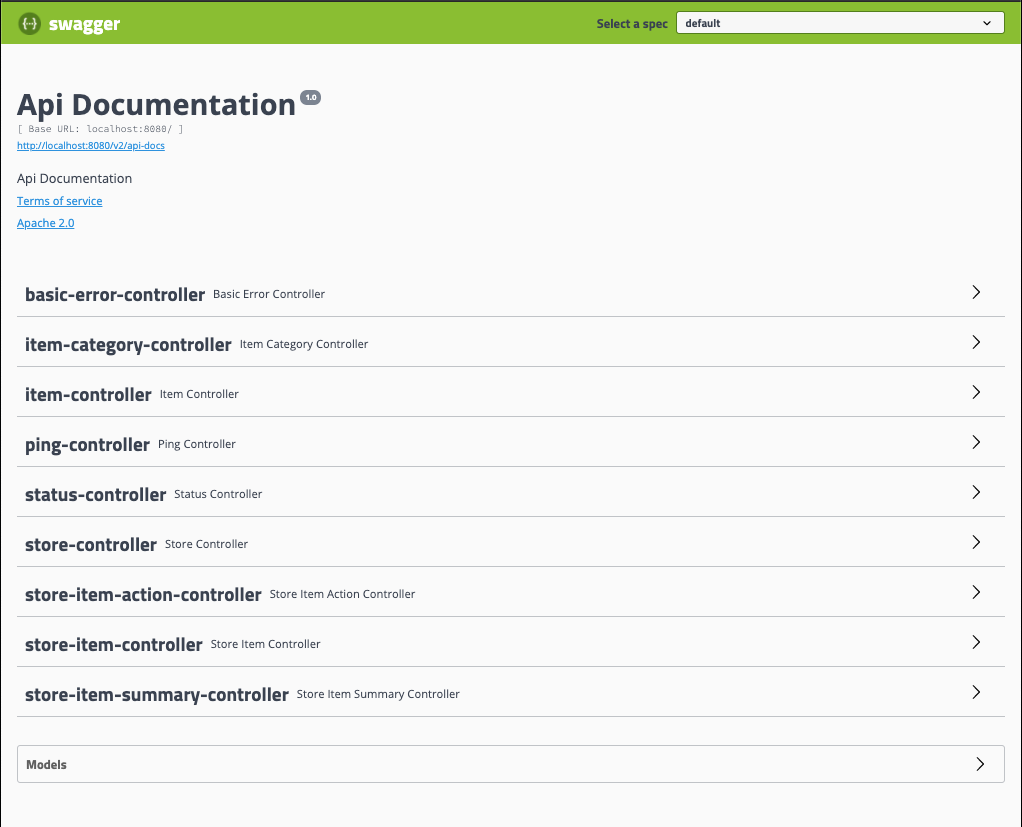
\includegraphics[width=10cm]{./assets/images/swaggerList.png}}
        \caption{The swagger documentation headings for all available controllers in the web service application.}
        \label{fig:swaggerList}
    \end{figure}
    \begin{figure}[H]
        \centering
        \frame{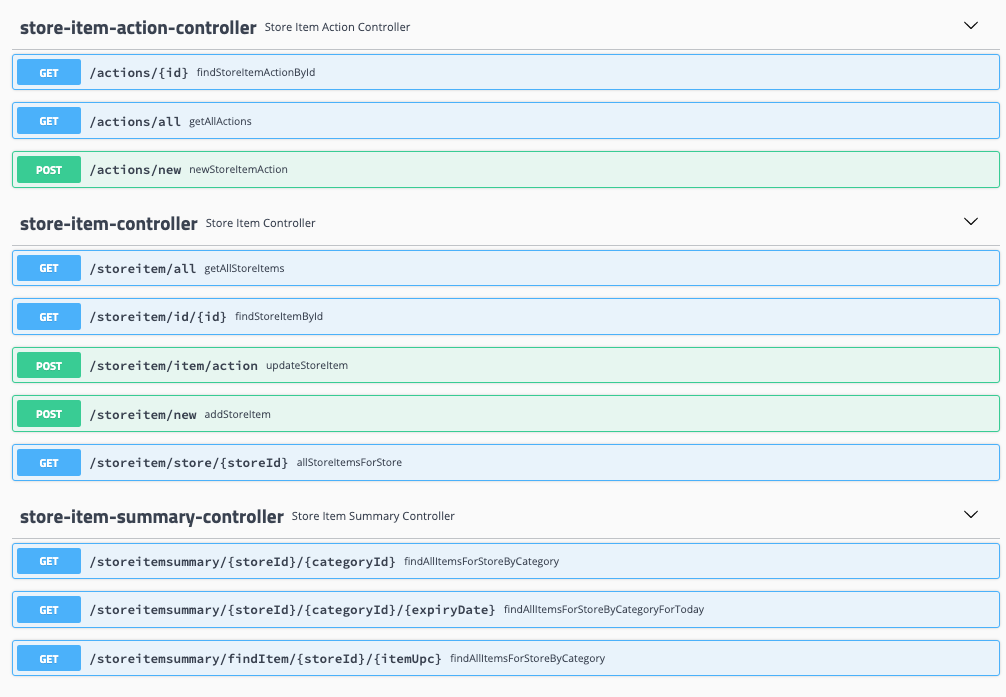
\includegraphics[width=10cm]{./assets/images/endpointDocs.png}}
        \caption{An example of the documentation of each of the endpoints within each controller.}
        \label{fig:endpointDocs}
    \end{figure}
    \begin{figure}[H]
        \centering
        \frame{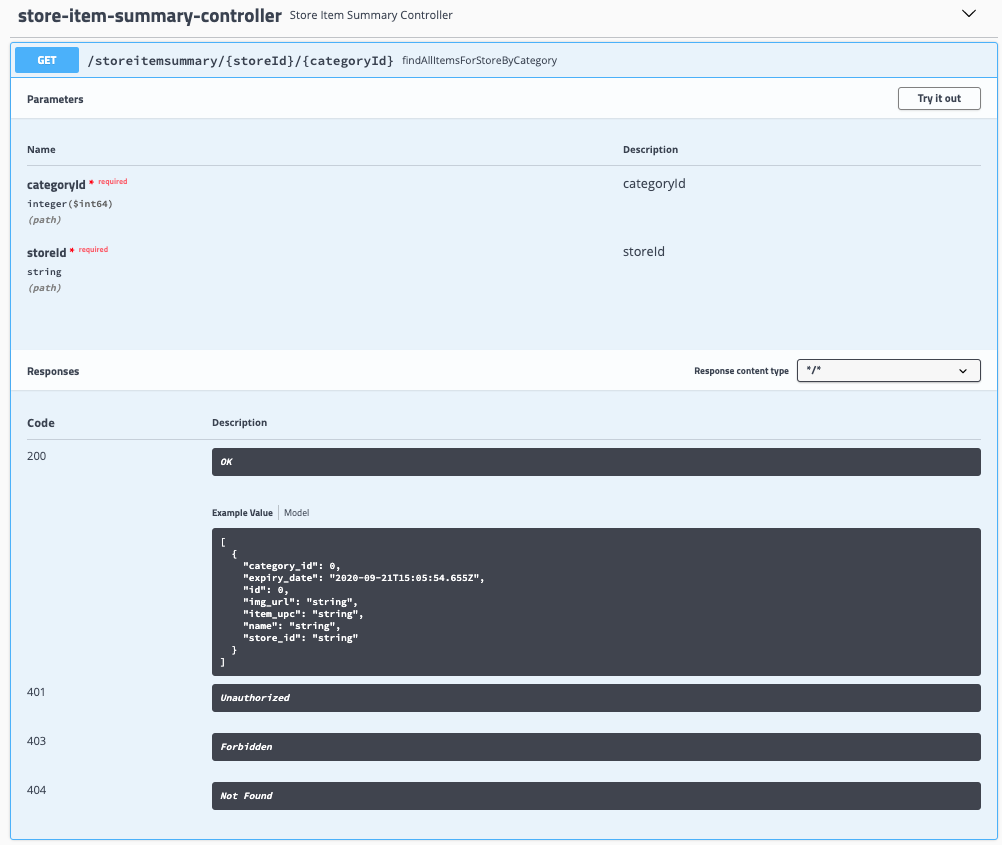
\includegraphics[width=10cm]{./assets/images/endpointExample.png}}
        \caption{A screenshot of the storeItemSummary controller endpoint, this includes the documentation for each potential response that the endpoint can return as well as the parameters which the endpoint expects to receive.}
        \label{fig:endpointExample}
    \end{figure}
    \begin{figure}[H]
        \centering
        \frame{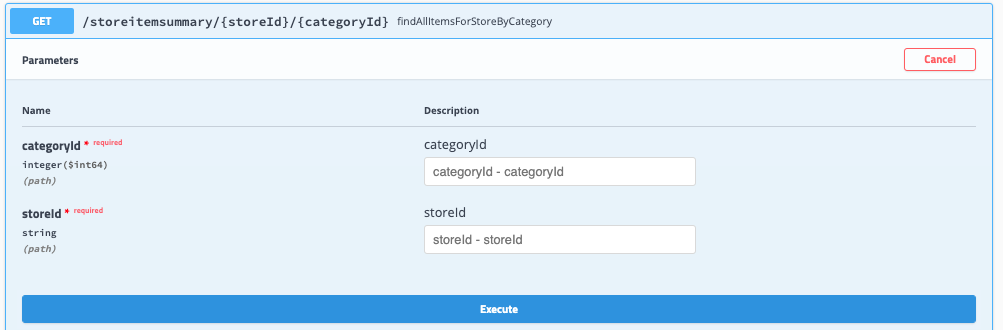
\includegraphics[width=10cm]{./assets/images/endpointTest.png}}
        \caption{A screenshot of how the endpoint can be tested within the swagger user interface.}
        \label{fig:endpointTest}
    \end{figure}
    \begin{figure}[H]
        \centering
        \frame{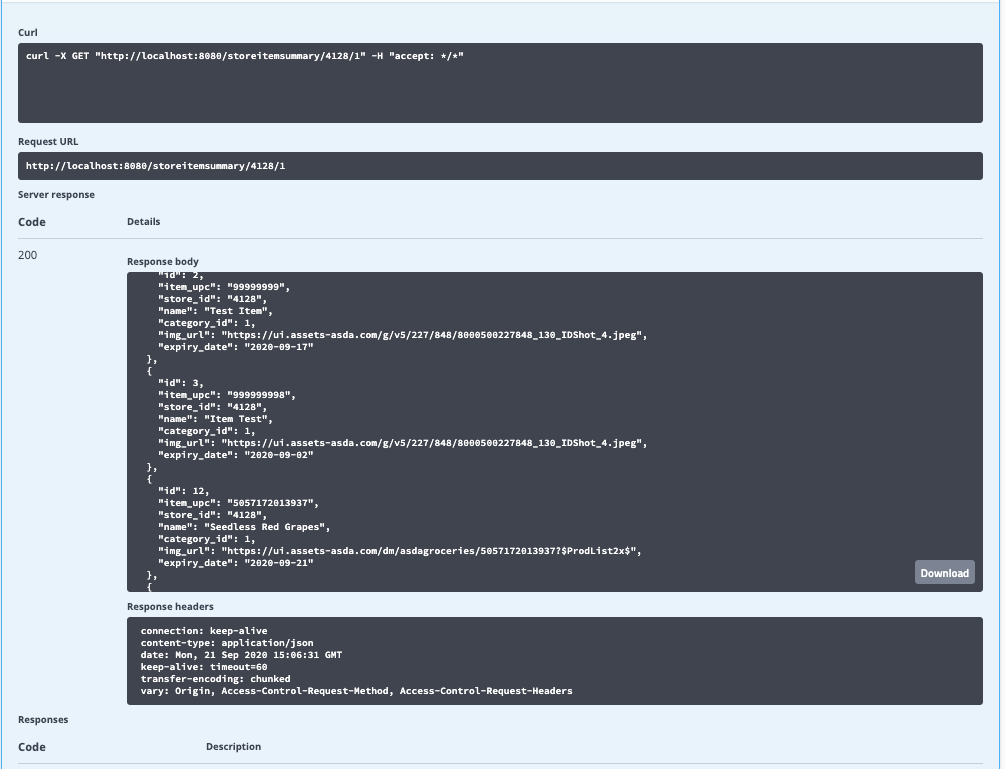
\includegraphics[width=10cm]{./assets/images/endpointTestResponse.png}}
        \caption{The response which is returned when a user successfully calls the endpoint via the Swagger UI.}
        \label{fig:endpointTestResponse}
    \end{figure}
\end{appendix}

\end{document}
